\documentclass{article}

\usepackage{verbatim}
\usepackage[dvipsnames]{xcolor}
\usepackage{blindtext}
\usepackage{titlesec}
\usepackage{graphicx}
\usepackage{fancyhdr}
\usepackage{caption}
\usepackage{listings}
\usepackage{color}
\usepackage{indentfirst}
\usepackage[hyphens]{url}
\usepackage[hidelinks]{hyperref}

\lstdefinelanguage{Golang}{
  alsodigit = {-},
  % Keywords as defined in the language grammar
  morekeywords=[1]{%
    break,default,func,interface,select,case,defer,go,map,%
    struct,chan,else,goto,package,switch,const,fallthrough,%
    if,range,type, continue,for,import,return,var},
  % Built-in functions
  morekeywords=[2]{%
    append,cap,close,complex,copy,delete,imag,%
    len,make,new,panic,print,println,real,recover},
  % Pre-declared types
  morekeywords=[3]{%
    bool,byte,complex64,complex128,error,float32,float64,%
    int,int8,int16,int32,int64,rune,string,%
    uint,uint8,uint16,uint32,uint64,uintptr},
  % Constants and zero value
  morekeywords=[4]{true,false,iota,nil},
  % Strings : "foo", 'bar', `baz`
  morestring=[b]{"},
  morestring=[b]{'},
  morestring=[b]{`},
  % Comments : /* comment */ and // comment
  comment=[l]{//},
  morecomment=[s]{/*}{*/},
  % Options
  sensitive=true,
  keywordstyle=\color{blue},
  commentstyle=\color{Green},
}

\lstset{
  basicstyle=\ttfamily,
  columns=fullflexible,
  frame=single,
  breaklines=true,
  postbreak=\mbox{\textcolor{red}{$\hookrightarrow$}\space},
}

\graphicspath{ {./images/} }

\definecolor{dkgreen}{rgb}{0,0.6,0}
\definecolor{gray}{rgb}{0.5,0.5,0.5}
\definecolor{mauve}{rgb}{0.58,0,0.82}

\newcommand{\subsubsubsection}[1]{\paragraph{#1}\mbox{}\\}
\setcounter{secnumdepth}{4}
\setcounter{tocdepth}{4}

\usepackage[a4paper, total={6in, 8in}]{geometry}
\setlength{\parskip}{0.8em}

\title{CM3070 Final Project - Preliminary Report}
\author{Esteban Garcia}
\date{ }
\pagestyle{fancy}
\fancyhf{}
\lhead{CM3070 Final Project - Preliminary Report}
\rfoot{Page \thepage}

\begin{document}
  \maketitle

  \tableofcontents

  \newpage
  \section{Introduction}

  For my project I'm going to be using the non-profit web application template.

  In the modern era of software development, the rapid adoption of third-party open-source libraries and containerised applications has revolutionised how software is built, deployed, and maintained. This shift has brought significant improvements on how we build software. However, it has also introduced new security challenges. As today's software supply chain increasingly depends on external dependencies, the potential attack surface for malicious actors has expanded dramatically.

  Software supply chain security aims to address the risks associated with this by ensuring that the integrity, provenance, and authenticity of software artifacts are safeguarded. High-profile supply chain attacks, such as SolarWinds and the exploitation of vulnerabilities like Log4Shell, underscore the critical need to secure software delivery and have demonstrated how a single compromised artifact can cascade through an ecosystem, affecting millions of users and causing substantial damage.

  To mitigate such risks, organisations and communities are adopting artifact management tools that enforce stricter security standards. These tools centralise the third-party dependencies and allow organisations to verify their origins, cryptographically sign artifacts and block software with known vulnerabilities.

  The Open Container Initiative (OCI) [1] compliance plays a pivotal role in this effort, as it promotes interoperability and consistency in how software can be packaged, distributed, and executed.

  OCI is a set of open-source standards designed to create a unified framework for container technology, focusing on interoperability and consistency across different container platforms.

  These standards were developed mostly with container technology in mind but starting with the OCI v1.1 specification, now it can be used to store any type of artifact as long as the specifications are followed.

  Making it suitable to support different artifact formats beyond just Container Images, bringing then the benefits of the OCI standard to them.

  Motivated by these considerations, my project aims to provide a secure platform for storing, managing, and distributing OCI artifacts.

  Using OCI as a storage layer allows for my project to leverage its capabilities to store any kind of software, this reduces compatibility issues and fosters consistency in development and deployment environments. 

  It ensures that artifacts are verifiable and tamper-proof through tools like digital signatures and hash-based verification.

  OCI-compliant tools integrate seamlessly with various ecosystem tools, such as container registries, Kubernetes, and CI/CD platforms. This interoperability makes it easier to share, store, and retrieve artifacts across diverse environments

  By following these standards, artifacts become more portable and adaptable, allowing organizations to easily move and deploy artifacts across cloud environments, on-premise systems, or hybrid infrastructures

  As there is a wide selection of different package formats in the ecosystem to prevent scope creep I will focus only on storage and distribution of Docker Images [2], Helm Charts [3] and PyPi (Python) Packages [4]. This last one is the only format that doesn't support the OCI protocol so a translation layer would need to be developed but it will serve as proof of the standard's capabilities to store and distribute any type of software.

  \section{Literature Review}

  \subsection{Similar Projects}

  This section provides an analysis of existing solutions, the two projects I'm focusing in here are JFrog Artifactory [5] and Harbor [6]. These platforms have two different approaches to artifact management and container registry functionality.
  
  JFrog Artifactory as a commercial, enterprise-grade solution with extensive support for different artifact formats, and Harbor as an open-source OCI compliant registry.

  This analysis will provide a foundation for understanding the design and implementation decisions behind the project, demonstrating how it aims to bridge existing gaps and contribute to the evolution of secure artifact management practices.

  \subsubsection{JFrog Artifactory (commercial product)}

  JFrog Artifactory is a commercial, universal artifact repository manager. It supports a wide range of package formats (e.g., Docker images, Maven, npm, PyPI) and integrates into CI/CD pipelines. It is well-known for its scalability, enterprise-grade features, and extensive integrations.

  The product offers no free version and is offered with both a cloud and a self-hosted solution. Its cloud-based product is not multi-tenant, meaning that JFrog needs to deploy standalone infrastructure for each customer, and its self-hosted solution is deployed and managed by the customer.
  
  Due to its closed-source nature, and lack of multi-tenancy features, this means that organisations can't be aware of any security vulnerabilities in the platform and patching of these would require JFrog to implement the fix, notify their self-hosted customers and then apply the patch to each Cloud instance administered by them.

  This last point is concerning as reported by Google in their latest report [7] we've been seeing the Time-To-Exploit metric being reduced from 32 days in 2021 \& 2022 to 5 days in 2023, and 97\% of them being exploited as zero-days vulnerabilities.

  Artifactory classifies itself as an `universal' artifact management platform, meaning it provides the capabilities to store any type of package format and new ones are being implemented all the time. But it uses its own Storage Architecture Layer and API that doesn't adhere to any open-source standard.

  Artifactory is OCI-compliant but the standard is not used as the storage layer for all of its supported format but rather only for OCI-artifacts only. 

  So this means that custom JFrog-developed libraries have to be used to interface with its APIs for administering artifacts outside of each format's native tooling.

  JFrog uses their own close-sourced static analysis vulnerability scanner called XRay [8], as it's a separate product it needs to be payed separately.

  At the same time signature [9] of uploaded packages is an `enterprise' only feature.

  Artifactory is a very complete solution but only accesible to those with a big budget and requires a lot of administrative effort to create a secure supply chain for an organization's software.
  
  \subsubsection{Harbor (open-source project)}

  Harbor is an open-source container image registry, built by VMware [10] and now part of the Cloud Native Computing Foundation [11]. It is designed to enhance container image security and improve efficiency in managing containerized environments.

  As it's an open-source project, Harbor benefits from community-driven development and transparency.

  In contrast to Artifactory, Harbor is fully self-hosted and requires the operator to deploy and administer its infrastructure without an multi-tenant cloud-hosted option.

  It's an fully OCI-compliant registry, this enables seamless integration with OCI-complaint tooling allowing developers/devops engineers to manage artifacts with either Harbor's Custom Tooling or native OCI tools. It only supports the upload of OCI artifacts, package formats that don't adhere to the standard can't be uploaded without additional custom automation.

  It provides vulnerability scanning by connecting to Trivy [12] or Clair [13], two open-source static analysis tools, these tools have to be deployed separately by the administrator.

  \subsubsection{Conclusion}

  Both projects have extensive support and can be used to secure an organisation's software supply chain.
  Even though Artifactory is OCI-compliant its underlying storage architecture is not based on that technology, increasing the complexity for its users and its commercial nature limits its usage only to those with deep enough pockets to pay for it.

  Harbor is fully OCI-compliant and open-source, it benefits from its transparency with the community but it focuses only on OCI/Container artifacts, doesn't support other package formats so it can't be used as a full solution to secure the supply chain.

  As to address the issues mentioned, my project will be taking a hybrid approach to both these solutions. As a non-profit project it will be fully open-source and the community will be able to contribute back to the project and be aware of any changes, but there will also be a cloud-hosted multi-tenant solution as to cater to more enteprise-based users that do not want to host their own solution and prefer a hands-off approach.

  Just like Harbor my project will be fully OCI-compliant built from the ground up following this specification, but unlike harbor it will support package formats outside the OCI-standard close to JFrog's offering.

  \subsection{Research Studies}

  In this section I evaluate different research studies that justify the development and usage of a project like the one I'm developing.
  
  William Enck and Laurie Williams define the Three of the Top Five Challenges in Software Supply Chain Security [14] as:

  \begin{itemize}
    \item updating vulnerable dependencies
    \item choosing trusted supply chain dependencies
    \item securing the build process
  \end{itemize}

  For a developer to be able to secure their software, they need to be aware of vulnerabilities on their dependencies, this process has to be automated so a platform that is aware of a software's dependencies has to be used for this.

  Choosing trusted supply chain dependencies is very important, what if a library your software is dependent on is deleted and someone takes the name? You don't only need to establish trust with the dependency you are using but also with the Package Index is coming from, most of the programming languages out there have some kind of public package index, PyPi for Python, NPM for NodeJS, there's good intentention behind these services but there's no guarantee that anything being uploaded there is safe as there is no vetting nor barrier to entry.

  Package Typo-squatting, a form of social-engineering attack that targets users who incorrectly type a package's name, is becoming more normal in public package indexes, a good example discovered by a member of the Python community named Bertus [15] who reviewed a malicious package named `pytz3-dev' seen in the Python package index (PyPi). This package targeted developers looking for the very popular `pytz' package, it executed malicious code that searched for a SQLite database used by Discord the popular chat application, this database is used by Discord to store user information locally but also it includes tokens used to authenticate the user against the service.

  So a developer should upload their dependencies to a trusted store where they have control over what goes in and what goes out.

  Recently the NSA released a paper on recommended practices for developers on how to secure the software supply chain [16], as part of their recommended Secure Development Practices, they recommend that all third-party libraries are uploaded to a secure repository where they can be analysed for vulnerabilities on an on-going basis and an audit log of upload and downloads of libraries is kept.

  \section{Design}

  My project (also referred to as `registry' in the report) operates in the domain of software artifact management, focusing on creation, storage, management, and distribution of software artifacts.
  
  This domain is critical for modern software development workflows, particularly in areas like:

  \begin{itemize}
    \item CI/CD Pipelines where the role of the registry here is to enable artifact storage and deployment automation.
    \item DevSecOps Workflows where the role of the registry is to provide signing to verify the artifact authenticity and allow integration with vulnerability scanners.
    \item Software Development Lifecycle where the role of the registry is to store and manage third-party softwaredependencies (e.g. python packages).
  \end{itemize}

  The registry serves as a central repository for managing artifacts in a secure, efficient, and interoperable way, promoting best practices in software delivery and supply chain security.

  \subsection{Target Users}

  The importance of an artifact management solution varies depending on the needs and responsabilities of the different user groups, from developers to operations and security teams. 

  These are the primary users of my project and how it adds value to each depending on their role

  \subsubsection{DevOps Engineers}

  The role of a DevOps Engineer is to automate software delivery pipelines, manage software deployments and ensure the infrastructure's reliability.

  Importance of an artifact management solution:
  \begin{itemize}
    \item Centralized Storage: Acts as a single source of truth for all deployment artifacts (e.g. Container images), simplifying their CI/CD pipeline automation
    \item Version Control / Artifact Management: Ability to manage multiple versions of artifacts
    \item Automation Support: Seamless integration with CI/CD tools for automated artifact pushing, pulling and deployment
    \item Immutable Artifacts: Ensure artifacts are tamper-proof once published
  \end{itemize}

  \subsubsection{Software Developers}

  The role of the software developer is to write and maintain the code for their business/company.

  Importance of an artifact management solution:
  \begin{itemize}
    \item Fast Dependency Download: Quick access to the packages they need for coding
    \item Artifact Publishing: A straightforward process for sharing new packages with their teams
    \item Consistent Environments: Ensure uniformity across development, testing and production environments
  \end{itemize}

  \subsubsection{Site Reliability Engineers (SRE)}

  Their role is to maintain and optimize the infrastructure where software is run on.

  Importance of an artifact management solution:
  \begin{itemize}
    \item High Availability: Provide consistent access to artifacts through replication and caching strategies
    \item Standardization: Enforce uniform deployment practices with controlled artifact usage in production.
    \item Operational Visibility: Offer detailed artifact usage, version history, and metadata for troubleshooting.
  \end{itemize}

  \subsubsection{Security Teams}

  Their role is to safeguard and ensure compliance with security standards.

  Importance of an artifact management solution:
  \begin{itemize}
    \item Artifact Integrity \& Signing: Verify that artifacts are authentic and untampered through cryptographic signing
    \item Vulnerability Scanning: Automatically identify security risks within stored artifacts as part of CI/CD pipelines.
    \item Access Control: Implement fine-grained permissions to restrict artifact access and modifications
  \end{itemize}

  \subsection{Project Features}

  Based on the needs of the previously mentioned users, my project will focus on the following features

  \subsubsection{OCI Compliance}

  As mentioned before my project will be leveraging the OCI specification for storage of artifacts, full compliance ensures that the registry supports multiple different types of artifacts, allowing diverse development teams to use a single solution. This standarization simplifies workflows and reduces compatibility issues, addressing both the centralization and standarization needs of DevOps Engineers and Software Developers.

  \subsubsection{OCI v1.1 Distribution Specification}

  This specification defines the API protocol to facilitiate and standardize the distribution of OCI artifacts, and it is design to be agnostic of content type. Container Images are the most prominent type but the protocol is open to any.

  One of the key features of OCI is being able to directly address storage by its content, this is done by calculating a `SHA256' digest of the content and always addressing it by the calculated digest. This allows for deduplication of binary data, and be able to share raw bytes with other uploaded artifacts.

  There are four different types of workflows as part of the specification:

  \begin{itemize}
    \item Pull - Clients are able to pull from the registry
    \item Push - Clients are able to push to the registry
    \item Content Discovery - Clients are able to list or otherwise query the content stored in the registry
    \item Content Management - Clients are able to control the full life-cycle of the content stored in the registry
  \end{itemize}
  
  \subsubsubsection{Terms Definitions}

  Before going in detail into the different categories, there are certain terms that warrant basic definitions:

  \begin{itemize}
    \item Repository: a scope for API calls on a registry for a collection of content (including manifests, blobs, and tags).
    \item Blob: the binary form of content that is stored by a registry, addressable by a digest
    \item Digest: a unique identifier created from a cryptographic hash of a Blob's content, normally SHA-256
    \item Manifest: A JSON document uploaded to the registry, it serves as an index, providing information needed to retrieve and assemble the layers and configurations that make up an artifact.
    \item Layers: A list of descriptors for the artifact, each pointing to a specific uploaded blob
    \item Push: the act of uploading blobs and manifests to a registry
    \item Pull: the act of downloading blobs and manifests from a registry    
    \item Tag: a custom, human-readable pointer to a manifest. A manifest digest may have zero, one, or many tags referencing it.
  \end{itemize}
  
  \subsubsubsection{Pull}

  This is the process of pulling manifest and blobs from the registry and typically the first step in pulling an artifact is to retrieve its manifest as it contains all the information on what blobs need to be downloaded.

  \subsubsubsection{Pulling manifests}
  
  This is done by performing a `GET' request to the registry to the URL \url{/v2/<name>/manifests/<reference>}

  Where `name' is the name of the repository and `reference' either the digest of the manifest or a tag.

  \subsubsubsection{Pulling blobs}

  This is done by performing a `GET' request to the registry to the URL \url{/v2/<name>/blobs/<digest>}

  Where `name' is the name of the repository and `digest' is the blob's digest

  \subsubsubsection{Checking for content existance}

  To verify for the existance of either a blob or a manifest a `HEAD' request to either the pull manifest or blobs URLs. A successful response would indicate that the content exists in the registry.

  \subsubsubsection{Push}

  This is the process of pushing manifests and blobs to the registry, and it works in the opposite order described previously, blobs are pushed first and the manifest last.

  \subsubsubsection{Pushing blobs}

  There are two ways to push blobs: chunked or monolithic. A monolithic upload happens as a single request to the registry, a chunked one consists of multiple upload request each one with a chunk of the blob. Each chunk is uploaded in order from start to finish.
  
  The client decides which type of push mechanism wants to use, but as a general rule of thumb, monolithic pushes will be used to upload small blobs and chunked to upload very big ones.
  But as this is a client-side decision the registry has to be ready to support monolithic upload of big blobs too. 

  There are two ways to push a blob monolithically, a POST request followed by a PUT request [18] or a single POST request [19].
  
  Chunk uploads are similar to the first option for a monolithic upload, the first POST request starts an upload session, then multiple PUT requests are made to the registry each one with a chunk of the blob, afterwards the upload is finalised by a last PUT request that also includes the cryptographic hash of the blob, this signals to the registry that the upload session is finished.

  When using chunk uploads all chunks must be uploaded in order, if not the registry will return an error.
  
  \subsubsubsection{Pushing manifests}

  To push a manifest a PUT request to the following URL is performed: \url{/v2/<name>/manifests/<reference>}

  Where `name' is the name of the repository and `reference' either the digest of the manifest or a tag.

  A manifest can have a different `Content-Type' depending on the type of artifact being pushed and it is used to identify the type of artifact server-side.
  
  Example `application/vnd.oci.image.manifest.v1+json' determines that the pushed manifest is for a OCI Container Image.

  This will be leveraged to identify what type of artifact we are receiving and also to create our own custom artifacts for those package formats that aren't supported out of the box by OCI.

  The request contains the cryptographic hash of the manifest used to reference it and it can optionally contain a tag too.

  \subsubsubsection{Content Discovery}

  These set of endpoints are used to fetch information from the registry about available artifacts.

  \subsubsubsection{Listing Tags}

  To fetch the list of tags a GET request to the following URL is performed: \url{/v2/<name>/tags/list}

  Where `name' is the name of the repository. The registry has to returned all available tags for the specified repository.

  \subsubsubsection{Listing Referrers}

  This is a new endpoint released as part of the OCI v1.1 specification [20]. A manifest can refer to a different manifest creating a relationship between the two, this endpoint allows for fetching all related artifacts for a specific manifest.
  
  This is good to attach things like signatures to an OCI artifact.

  To fetch the list of referrers a GET request to the URL is performed: \url{/v2/<name>/referrers/<digest>}

  Where `name' is the name of the repository, and `digest' is the digest of the manifest.

  Upon success, the response must be a JSON body with an image index containing a list of descriptors

  \subsubsubsection{Content Management}

  Content management refers to the deletion of blobs, tags, and manifests. These are optional endpoints that a registry may implement.

  \subsubsubsection{Authentication}
  
  The specification defines that registries may require authentication to interact with the registry.

  For this registries needs to return an `401 Unauthorized' error, including a `WWW-Authenticate' header with the URL for the login challenge and the Authentication scheme.
  
  The client then needs to send base64 encoded, basic authentication credentials to the endpoint and on successful response it will recieve back a token comformant with the authenciation scheme provided. 

  \subsubsection{Artifact format support}

  Uploading and downloading artifacts from the registry is the most basic yet important feature of the project, as all the target user's needs derive from this.

  There are dozens of recognized artifact formats out there across various ecosystems, my registry will only be supporting the following:

  \begin{itemize}
    \item Docker/OCI Images
    \item Helm Charts (via OCI)
    \item Python Packages (wheels)
  \end{itemize}

  This is to keep a well defined scope for the project given the available time. As a full OCI compliant API will be available it is possible for users to upload artifacts outside these defined formats.

  All uploaded artifact data will be stored within the registry.

  \subsubsection{Support for Native Tooling}

  Providing native tooling support allows users to integrate directly with the most widely used tools in their workflow, this prevents users from being `vendor locked' and requires minimal friction when integrating the artifact management solution with their already established CI/CD workflows.

  In the realm of this project this means supporting:

  \begin{itemize}
    \item Docker CLI for push and pull of container images
    \item ORAS (OCI Registry as a Storage) [21] CLI for push and pull of generic artifacts from OCI-compliant registries
    \item Helm CLI for push and pull of Helm Charts
    \item PIP (pip install packages) for downloading python packages from PyPi-compatible indexes
    \item Twine [22], a CLI tool for uploading Python wheels to PyPi-compatible indexes
  \end{itemize}

  \subsubsection{Multi-tenancy model}

  The project will function as a multi-tenant SaaS. A multi-tenant model means that a single instance of the registry will serve multiple independent organizations (tenants) while ensuring data isolation and security.

  In this project this model is structured around two hierarchical layers:

  \begin{itemize}
    \item Organisation: These represent administrative units within the project, serving as access control boundaries. Users must be members of an organisation to view, manage, or interact with the resources it contains.
    \item Registries: These are virtual segmentation units within an organisations and are where an OCI artifacts are stored. They provide a logical namespace for organizing and managing artifacts.
  \end{itemize}

  The key benefits for this come from all tenants sharing the underlying infrastructure where the registry is running, optimizing resource usage and reducing operational overhead. This makes the project easier to scale dynamically and more cost efficient.

  As OCI doesn't consider a multi-tenancy model in their specification, to address this limitation the organization and registry names will need to be scoped as part of all the API Endpoints, therefore as a requirement the users when using the registry they will need to prefix all of their OCI images with \url{<organization_name>/<registry_name>} this will allow the Registry API to identify to which organization and registry the uploaded artifacts belongs to as to be able to maintain its multi-tenancy and apply the appropiate access control.
  
  \subsubsection{Authentication}

  Security is an key aspect here, so we need to have strong access control to only allow uploads or downloads of artifacts to users that are authenticated and have the right permissions.  
  
  The project will be secured using the Bearer authentication scheme [23]. All users will need an valid JWT Token [24] to successfully authenticate against the API.

  To avoid storing sensitive credentials that could be leaked in the case of a data breach, I will instead be leveraging AWS Cognito [25] an OAuth2 provider [26], with this I don't need to store sensitive credential data and can just verify incoming if an incoming JWT token was issued by my AWS Cognito User Pool.

  This means that signup and, by default, authentication happen outside the control of the application too. This is fine for the Web UI but for OCI-compliant tooling we need to provide a login endpoint, receive the user's credentials and exchange them for a JWT token. Luckily OAuth2 has a flow designed for this called the username-password flow [27] and Cognito supports it, so I will be leveraging this functionality for credentials exchange on the OCI login endpoint. The usage of this authentication flow is discourage as it means the application has to recieve user credentials directly, but unfortunately for now most OCI-tooling doesn't have support for OAuth2-compatible authentication mechanisms. See \hyperref[sec:appendix-a]{Appendix A} for OCI authentication flow integrating cognito.

  The application would still need to at least be aware of user signups and maintain a User profile to be used for RBAC authorization, as signup and signin occur completly outside the control of the application I will be leveraging Cognito Triggers to execute an AWS Lambda function that will send a message to an SQS queue, a background worker will consume these messages and create an entry on the database.

  \subsection{Access Control}

  With authentication sorted, the project has to deny access to an authenticated user to resources it doesn't have the necessary permissions for.

  I plan on leveraging an RBAC architecture to control an user's access to resources within the application. A user could have any of these three roles within an organisation:
  \begin{itemize}
    \item Viewer: A user with viewer role will only have read-only access to the resources to the organisation it belongs to. This means it will only be able to list registires and artifacts and pull them.
    \item Writer: A user with the writer role has all the permissions of the viewer role, plus it can push and delete artifacts
    \item Admin: A user with full administrative control of all resources within the organisation, it has all the permissions of the writer role and it can manage members of the organisation.
  \end{itemize}

  \subsection{Artifact Storage}

  As the backbone of the project is storing Artifact Blobs and their availability for my users is the most important aspect of the project, I will be leveraging the AWS Simple Storage Service (S3) [27] as my base storage layer.

  S3 is a highly scalable and durable object storage service by AWS, it has 99.999999999\% durability and 99.99\% availability [28], it also has features like encryption, lifecycle management and object versioning making it a perfect solution for storing OCI artifacts in a safe manner.

  As S3 has a really powerful API to query for files, I'm also going to be leveraging these capabilities to know if a blob exists or not without having to store this data in the application's database.

  Both uploaded Blobs and Manifests will be stored on an S3 bucket. Given the nature of how OCI uploads work, there will be a 2-tier approach to storing them.

  As explained in the OCI section of this design, the upload of a blob works in the following way:

  \begin{enumerate}
    \item An upload session is initiated for a specific OCI artifact in a repository.
    \item The blob data is uploaded
    \item The upload is finished and the client sends the blob digest
  \end{enumerate}

  We receive the full data of the blob before knowing its digest, and given the content addressable storage of OCI the application has to store the blob alongside its digest on S3 to be able to address it, so to circumvent this the application will do the following:

  \begin{itemize}
    \item When an upload session is requested by the client, a random ID will be generated.
    \item In-flight blobs, these will be blobs that we received but don't know the digest yet, will be stored in S3 under a key called `in-flight'
    \item Once the upload session is finished and the application receives the digest for the blob, it will leverage the S3 API to move the file to the final location using the digest as key.
  \end{itemize}

  See \hyperref[sec:appendix-b]{Appendices B, C and D} for upload flows.

  As S3 has a limit for a single file upload of 5 GB, OCI artifacts, specially container images can very quickly reach that limit. So to account for this the multipart upload API [29] will have to be used, with this objects up to 5TB can be uploaded. The way the application will manage this is by creating an multipart upload session when an OCI client requests a new upload session and finalise it when the OCI upload session is finalised too.

  With the data stored on S3, I can then create self-expiring presigned[30] links and redirect the user directy to S3 to download a blob or manifest without having to keep a connection to my own application, reducing load and making it more cost-effective to run. See \hyperref[sec:appendix-e]{Appendix E} for blob download flow.

  \subsection{Implementing the PyPi interface}

  As mentioned before my project is based on the OCI protocol, but as I would like to expand its functionality to also support the PyPi index repository interface to store and serve python packages.

  As PIP is not an OCI-compatible package manager, I need to implement an server-side interface to translate from the OCI protocol to the expected PyPi index responses.

  There are two endpoints that need to be created for this.

  \subsubsection{Upload API}

  The PyPi Upload API [31] endpoint is the endpoint that tools such as Twine use to upload packages to PyPi.

  This is a POST request to the base endpoint of the configured repository URL in Twine, the users configure this in their `~/.pypirc' file, it looks something like this:

  \begin{lstlisting}
    [distutils]
    index-servers =
      ociregistry
    [ociregistry]
      repository: https://url/api/v1/<organization>/<registry>/python
      username: username
      password: password
  \end{lstlisting}

  Where \url{https://url/api/v1/<organization>/<registry>/python} is the registry-defined URL a user has to configure for uploads. In the case of my project the URL has to indicate the organization and registry where the user intends to upload their packages and indicate their credentials too.

  When initiating an upload, twine uploads the `.whl' file, which is the python-built artifact.

  To interface with OCI, I plan on leveraging the ORAS (OCI Registry as Storage) library for simplicity. This library repurposes OCI-compliant registries as generic storage system for storing any type of artifact and is one of the native tools that I plan to support, so by using this I adhere with the OCI-compliant nature of my project and I'm able to reuse all the upload and download flows that OCI exposes with their endpoints.

  I will be using `application/vnd.python.artifact' as custom `artifactType' for python packages, this will allow the registry and users to query for python packages.

  See \hyperref[sec:appendix-f]{Appendix F} for Python Upload flow diagram.

  This will automatically expose the Python package via the OCI APIs. But for pip to be able to discover this package the application needs to implement the Simple Index Repository API endpoint.

  \subsubsubsection{Anatomy of the WHL File}

  A ptyhon wheel file is basically a zip file, on extraction we usually find two folders, one containing the python code of the library to be used by a project referencing it as a dependency, and the `dist-info' folder.

  This folder contains metadata that needs to be exposed in the Simple Repository Index response and is used by pip to determine python version requirements among other things.

  This metadata is stored inside a file called `METADATA', and the data within it follows the RFC 5322 Internet Message Format [32], used in e-mails today. As it is a widely use format it is very simple to parse.

  The metadata will be stored as annotations within the OCI Manifest. See \hyperref[sec:appendix-g]{Appendix G} for an example on the structure of the OCI Manifest for a python package.

  \subsubsection{Simple Repository API}

  The Simple Repository API is an HTML index, and is how a Python package repository exposes to clients (like pip) the available packages and available version of each package.

  The implementation of this API is based on the PEP-503[33] Python Enhancement Proposal specification.

  Within a repository, the root URL MUST be a valid HTML5 page with a single anchor element per project in the repository. The text of the anchor tag MUST be the name of the project and the href attribute MUST link to the URL for that particular project. As an example. See \hyperref[sec:appendix-h]{Appendix H} for an example.

  Below the root URL is another URL for each individual project contained within a repository. This URL must respond with a valid HTML5 page with a single anchor element per file for the project. The href attribute MUST be a URL that links to the location of the file for download, and the text of the anchor tag MUST match the final path component (the filename) of the URL. The URL SHOULD include a hash in the form of a URL fragment with the following syntax: `\#\textless{}hashname\textgreater{}=\textless{}hashvalue\textgreater', where `\textless{}hashname\textgreater' is the lowercase name of the hash function (such as sha256) and `\textless{}hashvalue\textgreater' is the hex encoded digest.
  See \hyperref[sec:appendix-i]{Appendix I} for an example.

  To implement this in my project, the endpoint would need to discover all OCI artifacts with the custom `mediaType' created on upload and dinamically generate the HTML response, this will allow for PIP to download Python packages stored on an OCI-compliant repository.

  \subsubsection{Twine Authentication}

  As twine is not an OCI-compliant tool it doesn't follow the authentication flow previously discussed. It uses Basic authentication credentials on each request, luckily this method is already used for the initial credential exchange for the OCI login endpoint.

  The biggest downside is that each request would need to validate credentials with AWS Cognito, calling an external service on each request will more than likely impact the 
  response time of the service.

  \subsection{Database Design}

  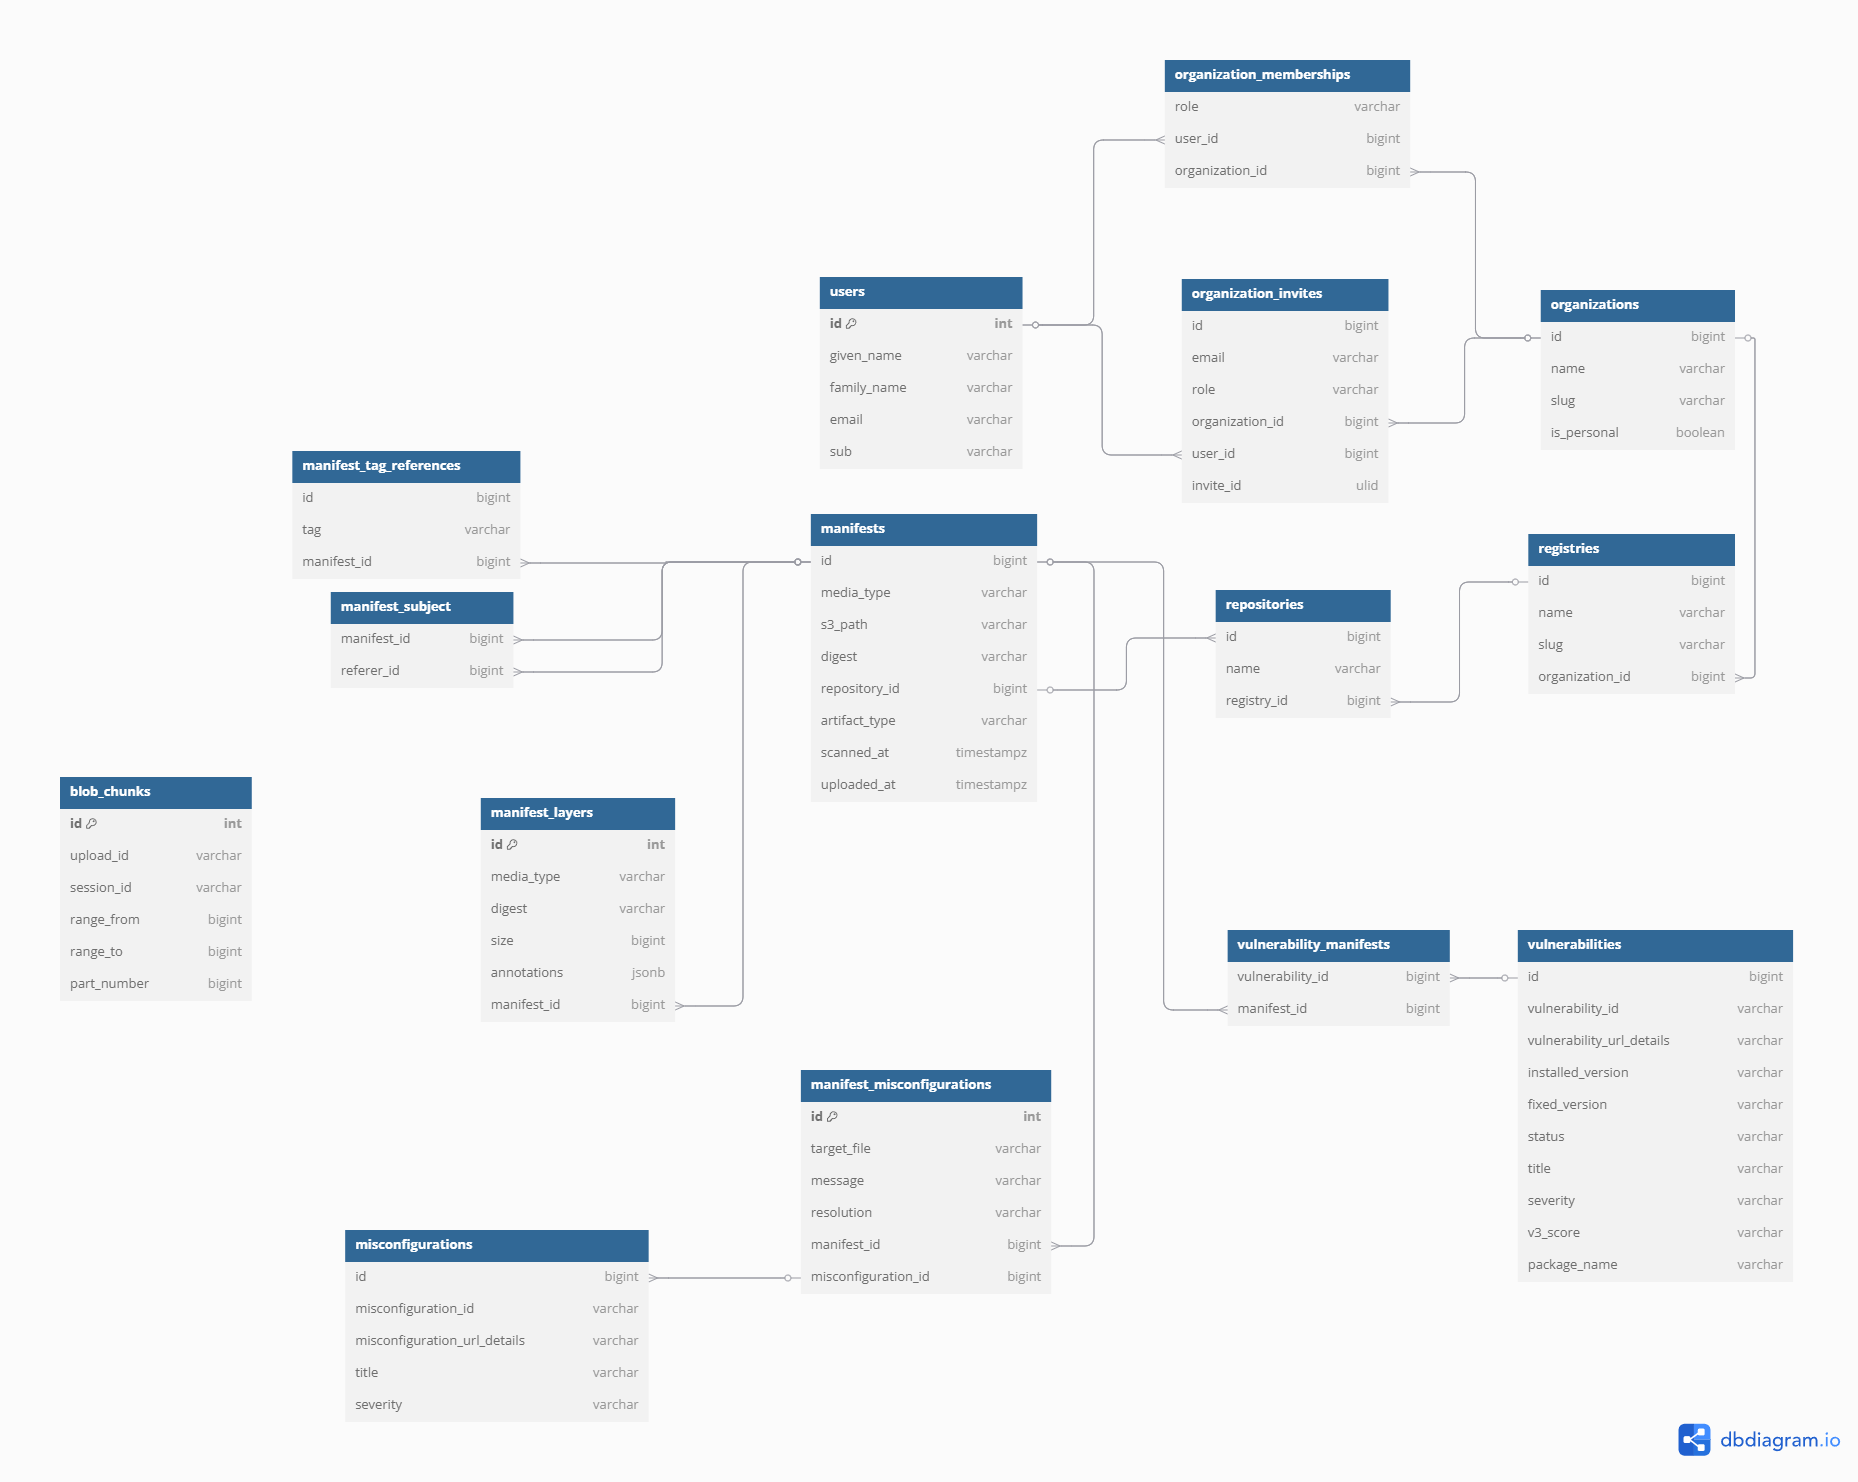
\includegraphics[scale=0.35]{db.png}

  \subsection{Gantt Chart}

  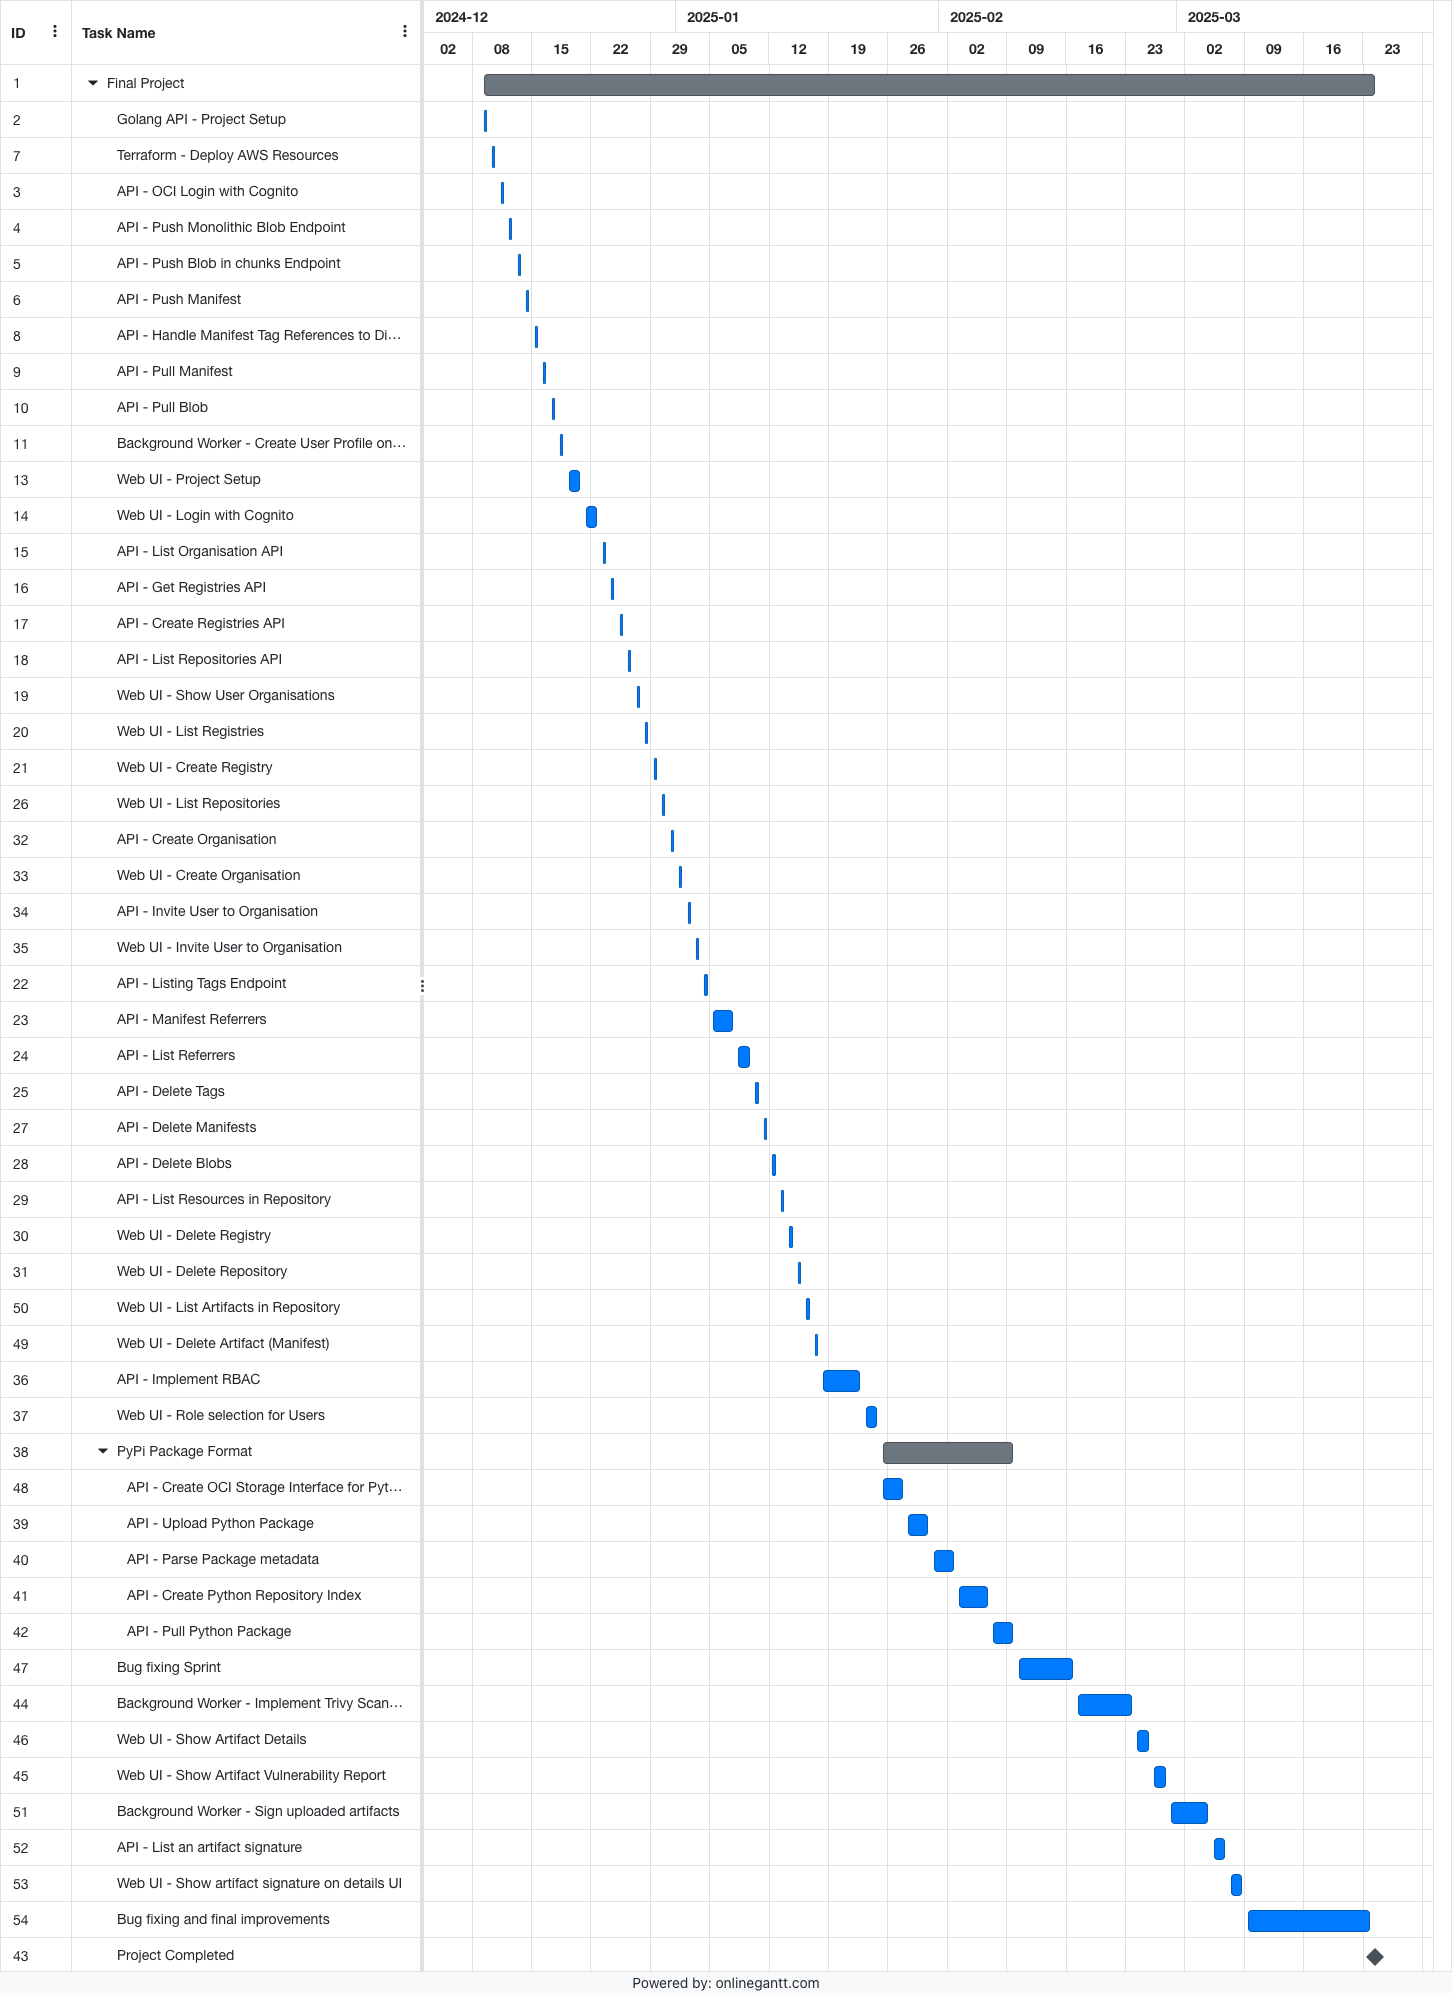
\includegraphics[scale=0.27]{gantt.png}

  \section{Implementation}

  \subsection{Technology Stack}

  For my tech stack I've selected the following:
  \begin{enumerate}
    \item GoLang[35] for Backend APIs
    \item PostgreSQL[36] for Database Engine
    \item NextJS[37] for Web UI Framework
    \item AWS S3 as storage layer
    \item AWS Cognito as OAuth2 Provider
    \item Trivy Scanner for vulnerability scanning
    \item Terraform[38] for Infrastructure as Code
    \item Terraform Cloud for orchestrating the deployment of AWS infrastructure
  \end{enumerate}

  I selected Golang as the main programing language for the backend API for the following reasons:

  \begin{itemize}
    \item Performance: Golang is a compiled language, offering high performance and low latency, which I think is critical for handling a large volume of artifact storage operations.
    \item Concurrency: It has built-in support for concurrency through goroutines, making it perfect for handling multiple simultaneous requests without the need for an external webserver.
    \item Ecosystem: The OCI ecosystem and related libraries are mostly implemented in golang, making it easier for my project to include them as dependencies if needed
    \item Simplicity: I find its syntax clean and easy to read, write and maintain
  \end{itemize}

  NextJS is a React-based framework with support for Server-side rendering, I selected this framework due to my familiarity with React thanks to the CM3050 Mobile Development module, and because its server-side rendering allows me to build a more secure WebUI, any sensitive data can be handled server-side and won't leak to the client unneccesarly. This also makes the frontend much more performant as complicated React components can be rendered on a server with more resources.

  As explained in the Design section of this report, I will be leveraging cloud services from AWS.
  Managing the creation and update of these services manually can be a tedious task, this is where Terraform comes into the picture. Terraform is an infrastructure as code tool that allows to define cloud infrastructre using declarative configuration files, this helps with managament of cloud resources and also allows for easier reproducibility of environments.

  \subsection{High-level Architecture Diagram}

  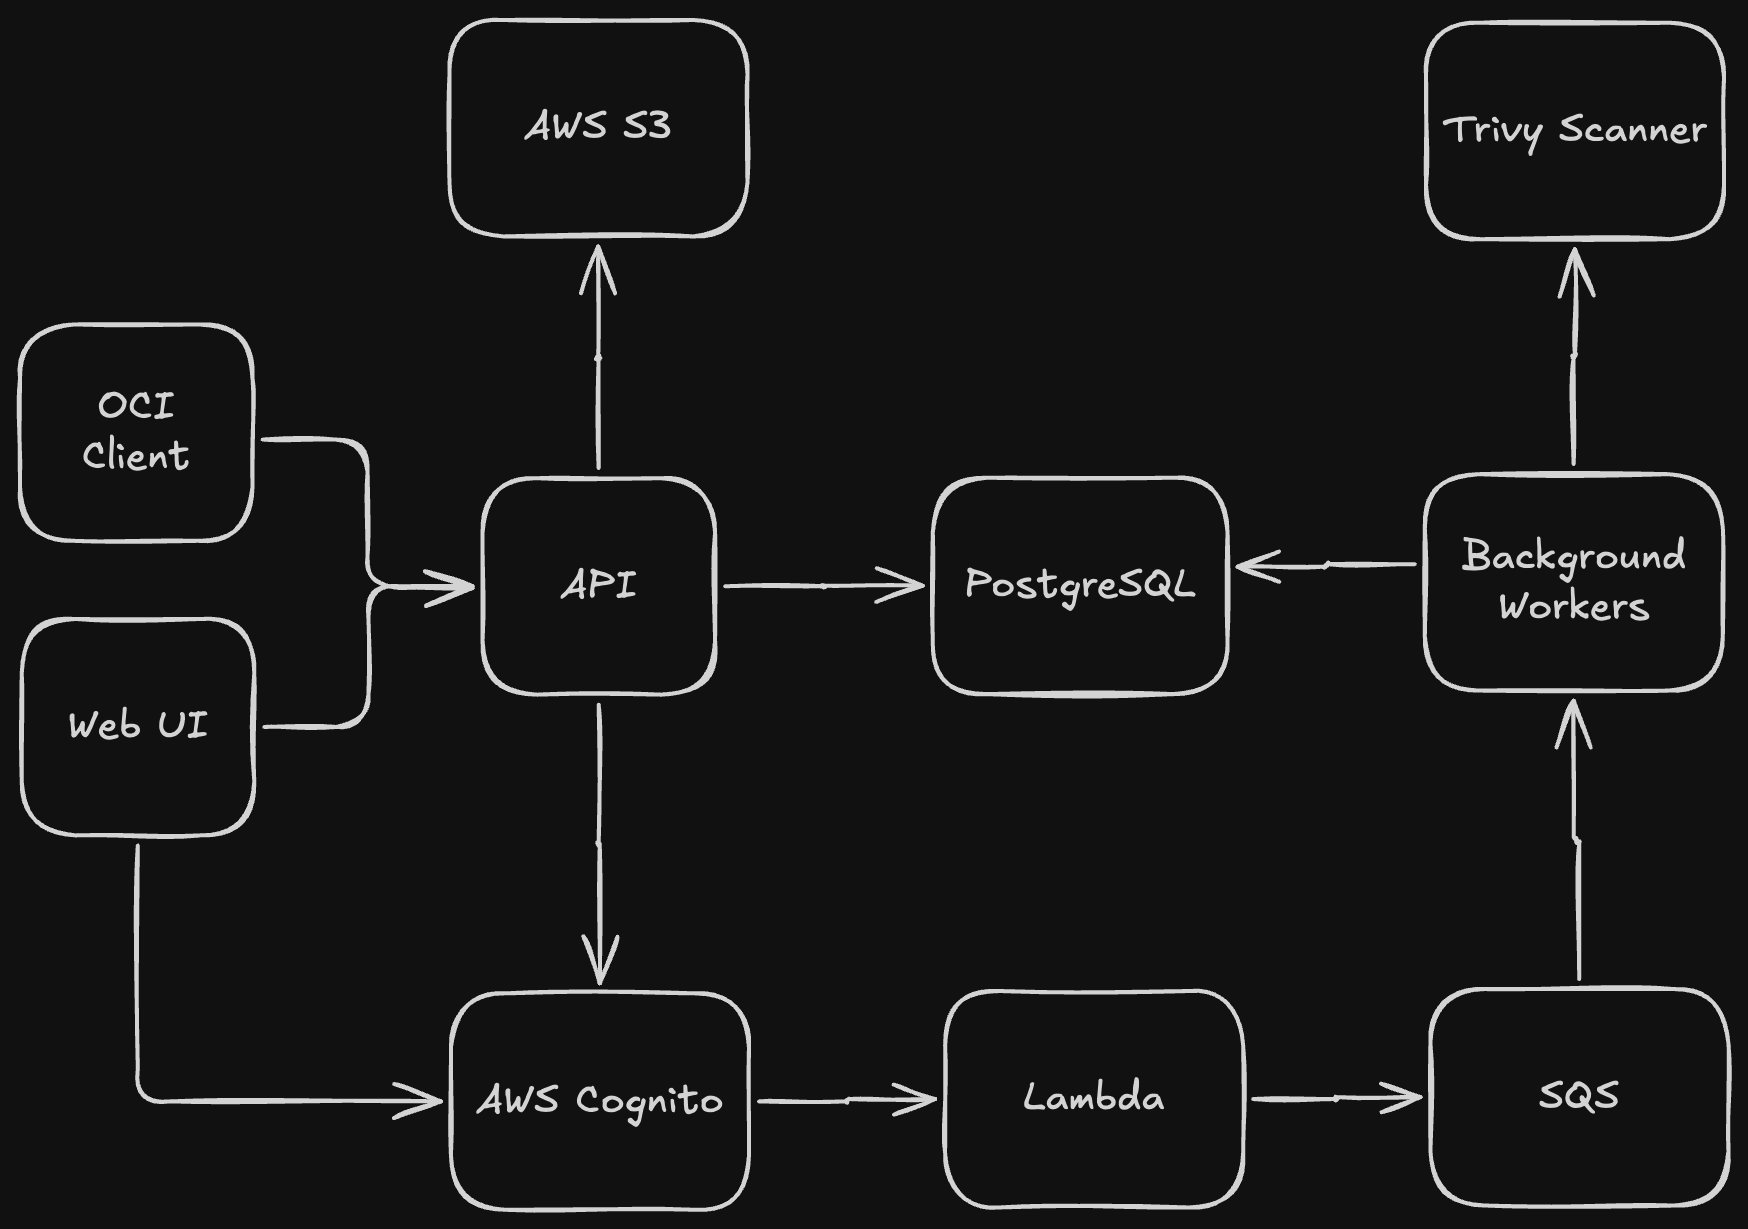
\includegraphics[scale=0.25]{architecture.png}

  \subsection{Software Development Lifecycle}
  I'll be using Git as a Version Control system, I will have 3 different projects.

  \begin{enumerate}
    \item Backend API Source Code
    \item Web UI Source Code
    \item Terraform Code
  \end{enumerate}

  All changes to the 3 different projects will be submitted via the Merge Request system in Git, this will allow for cleaner commit history and traceability of changes, and it will be paired with a CircleCI pipeline that will automatically execute any unit tests available and block the change to be merged if they fail.
  
  For organising work tasks I'm going to use Trello. I will be doing 1-week sprints, keeping them short will allow me to better plan work and break down stores to simpler tasks that can fit in one week.

  At the end of each sprint I will do a review of all the commited work, test each feature individually, create stories for Bugs if any are found and plan the next sprint.

  As I'm the only developer involved in the development it will be very hard to not be baised on all the submitted changes, to try to mitigate this I'm going to be leaning on the tooling provided by the go language to lint the code and perform static analysis of the changes. This will be included in the CircleCI pipeline and block me from merging changes if I don't solve the outstanding issues.

  \subsection{Managing Database Changes}

  In the golang application I will be using the EntGO[39] entity framework. This is a simple ORM for querying a database and mapping data to Golang Structs.

  EntGO allows me to easily model the database schema programmaticaly using Go code, this integrates nicely with Atlas[40] a tool to auto-generate SQL migration files based on the EntGo schema.

  This allows me to keep database changes alongside the code of the application and keep it under source control.

  Based on an EntGo schema like:

  \begin{lstlisting}
    package schema

    import "entgo.io/ent"

    // User holds the schema definition for the User entity.
    type User struct {
        ent.Schema
    }

    // Fields of the User.
    func (User) Fields() []ent.Field {
        return nil
    }

    // Edges of the User.
    func (User) Edges() []ent.Edge {
        return nil
    }
  \end{lstlisting}

  Atlas will create the following SQL migration:

  \begin{lstlisting}
    CREATE TABLE `users` 
    (
      `id` bigint NOT NULL AUTO_INCREMENT, PRIMARY KEY (`id`)
    ) CHARSET utf8mb4 COLLATE utf8mb4_bin;
  \end{lstlisting}

  Atlas will also be applying the migration changes to the database.

  \subsection{Repository Pattern}

  Keeping application along with database logic makes applications more complex, hard to test and maintain. So to avoid this I will be using the Repository Pattern to query the database.

  The repository pattern is a way to abstract the data layer and encapsulate data access logic into a dedicated layer. A repository will act as a middle layer between application logic and the data mapping layers, in EntGo the data mapping layer would be the Entity Schema.

  Each Database Schema model will have its own repository used by the application to CRUD information on the database.

  See \hyperref[sec:appendix-j]{Appendix J} for an excerpt of one of the application's repositories.

  Each repository is represented by its own struct, this contains any dependencies required by the repository, usually the shared database connection. They are instantiated as a pointer when the application starts, this is to avoid unneccesary copies reducing the memory footprint and contributing to the application's performance.

  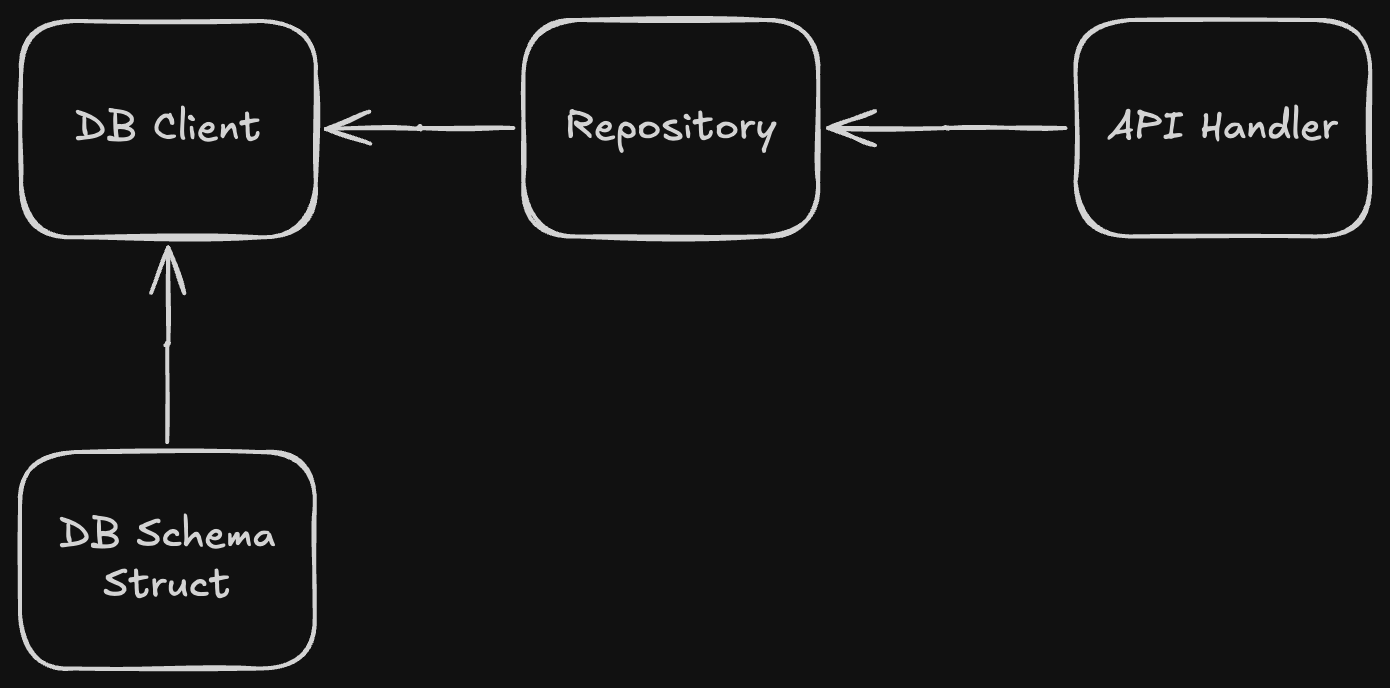
\includegraphics[scale=0.30]{repository_pattern.png}

  \subsection{HTTP Handler Pattern}

  The application uses `chi'[42], a lightweight composable router for building HTTP services, it is not a framework but rather it just focuses on HTTP routing and middleware.

  It has an unopinionated structure, which is beneficial for this project as it offers more flexibility needed to support both OCI-compliant endpoints mixed with the multi-tenancy requirements defined in the Design section. For this I needed to create custom routing logic which would have been more difficult to achieve with a framework with an opinionated structure.

  In Go the handler pattern is a common design approach that leverages the `net/http' package abstractions that are also used by `chi'. It is used to create modular, testable and composable code for handling HTTP requests.
  
  Each handler is represented by its own struct, the struct must implement the `http.Handler' interface, this is achieved by having all methods that serve requests implementing the `ServeHTTP(w http.ResponseWriter, r *http.Request)' interface.

  This allows to have separation of concern for API groups, this encapsulation promotes better organization and easier testing. It also allows for dependency injection, each handler will define all the dependencies it needs.

  See \hyperref[sec:appendix-k]{Appendix K} for an excerpt of one of the application's handlers.

  \subsection{Middlewares}

  A middleware in web development is a function that intercepts HTTP requests before they reach to the main route handlers.

  They encapsulate common logic that can be applied to multiple routes reducing code duplication.

  In my project I've created three different middlewares to perform certain validations and checks before the request is handover to the handler for processing.

  \begin{itemize}
    \item `ExtractBasicCredentialsMiddleware': For endpoints where basic authentication is required, such as the OCI login and all of the PyPi-related routes. This middleware validates against AWS Cognito the credentials and exchanges them for a JWT Token
    \item `JWTAuthMiddleware': For endpoints where Bearer authentication is required, this endpoint verifies that the JWT token recieved is valid and extracts information about the user that can be used by handlers
    \item `OrganizationMiddleware': As explained before in the multi-tenancy model of the project, organisations are the administrative units that user belongs to and where all resources live under. For all organization-scoped endpoints, this middleware checks that the authenticated user has access to the organisation.
  \end{itemize}
  
  Depending on the route group, not all of these middlewares are executed, but in some scenarios they are all chained together executed in order.

  See \hyperref[sec:appendix-l]{Appendix L} for an example of the middleware flow for a python index request.

  \subsection{Web UI}

  As mentioned in the Technology Stack section of the report, I'm using NextJS a React-based framework to create the web UI. As the target users of my project will mostly be using CLI tooling to interact with it, there won't be significant development of UI-based features.

  To accelerate development, I'm using the free to use ShadCN UI[43] components.

  The Web UI currently has the following features:
  \begin{itemize}
    \item WebUI can Signup and Login users via AWS Cognito
    \item A user can switch between organisation on the WebUI
    \item List of registries
    \item Create a registry
    \item List of repositories
  \end{itemize}

  There are still some features that I need to include that haven't been started yet:
  \begin{itemize}
    \item Creation of new organizations
    \item Visualization of artifacts in a repository
    \item Invite users to an organization
    \item Manage access control for a user
  \end{itemize}

  See \hyperref[sec:appendix-m]{Appendix M} for screenshots of the UI.

  \section{Evaluation}

  I will be testing my project in 3 different ways.

  Being fully OCI-compliant is the backbone of my idea, without being comformant with the specification I won't be able to develop the other features that depend on it. The OpenContainer Initiative provides an automated test suite[41] that developers can use to understand how compliant their projects are with the distribution specification, and outputs an HTML report. I will be using this test suite to identify gaps and issues on my OCI interface.

  I will be creating unit tests for all the developed APIs on the backend to validate each individual component in it. A CircleCI project will be used to automate running these tests on each commited change, this will ensure that new changes don't break existing functionality.

  Finally I will be doing some usability testing with some of my target users to evaluate the UX and interface design, the feedback gathered will be used to fix bugs and improve the different features.

  To test e2e functionality from a user perspective I will be using:

  \begin{itemize}
    \item Docker CLI
    \item ORAS CLI
    \item Helm v3 CLI
    \item Twine for upload of python packages
    \item PIP for installing python packages
  \end{itemize}

  \subsection{OCI conformance test suite}

  When developing the OCI implementation in my project, I heavily relied on the OCI test suite to identify bugs and understand gaps in my implementation to become fully OCI-compliant.

  This suite consists of 79 tests that are executed against a registry's API, these tests are divided into the four different workflows as explained in the Design section of the OCI v1.1 Distribution Specification

  \begin{itemize}
    \item Pull - Clients are able to pull from the registry
    \item Push - Clients are able to push to the registry
    \item Content Discovery - Clients are able to list or otherwise query the content stored in the registry
    \item Content Management - Clients are able to control the full life-cycle of the content stored in the registry
  \end{itemize}
  
  As of the time of writting the project is fully OCI-compliant. See \hyperref[sec:appendix-n]{Appendix N} for a screenshot of the test suite.

  \subsection{Unit Testing}

  At this moment the projects lacks unit testing, and this will be something I'm going to be working on the next couple of weeks. I made the conscious decision to not follow a test-driven development workflow as when I started the development there were some areas of the implementation of my project that were not very clear to me at that point in time.

  In hindsight delaying the creation of these has been a mistake as I've found software regression when working on new features

  \subsection{User Testing}

  I've reached out to people I know in the DevOps space and asked them to give the prototype of my project a try. I was able to get 2 people to try it out and give me some feedback based on their experience.

  For this I sent a survey with a couple of questions:

  \begin{itemize}
    \item How easy was it to start using the registry?
    \item How well would this registry integrate with your current CI/CD pipeline?
    \item Are there any features or functionalities you felt were missing or could be improved?
    \item Were there any error messages or unexpected behaviors?
    \item What is the one thing you would change or improve immediately if you could?
  \end{itemize}

  They both stated that because they had experience with similar technologies, starting to use the registry was easy and integration with an existing CI/CD pipeline would be trivial given the compliance with the OCI standard. But the lack of documentation and onboarding procedure on the UI would make it harder for someone not as experienced.

  In terms of missing functionality one of them mentioned the lack of OIDC Connect authentication for CI/CD pipelines and that even though it is soon to be developed, the lack of access control is very important.

  None of them had any unexpected issues, and for the last question the most important thing missing is visibility of uploaded artifacts via the UI

  So even though the UI is not something they feel is very important for their day to day workflows, the lack of visilibility of stored artifacts is, and is not something that is very well solved by current OCI-compliant tooling.

  \section{Conclusion}

  This project set out to develop an OCI-compliant registry to meet the modern demands of secure artifact management but also expands the scope of OCI beyond container images. 
  By leveraging the OCI specifications alongside tools like ORAS, the registry supports multiple artifact formats—including Docker images, Helm charts, and Python packages.

  The design of the registry was heavily influenced by the need to secure software delivery pipelines in an era of increasingly sophisticated supply chain attacks. This ensures that developers can reliably store, manage, and distribute software artifacts while maintaining high standards of security and operational efficiency.

  Future work could explore the support for additional artifact types, deeper integration with vulnerability scanners, and deny package downloads based on user-defined policies to allow them to do things like block download of packages with critical known vulnerabilities.
  
  Ultimately, this project lays a foundation for advancing secure software supply chain practices and promoting safer software consumption in organisations.

  \newpage

  \section{References}

  [1] `OpenContainer Initiative', \url{https://opencontainers.org/}
  
  [2] `Docker Inc.', \url{https://docs.docker.com/get-started/docker-concepts/the-basics/what-is-an-image/}

  [3] `Helm', \url{https://helm.sh/docs/topics/charts/}

  [4] `PyPi', \url{https://pypi.org/}

  [5] `JFrog Artifactory', \url{https://jfrog.com/artifactory/}

  [6] `Harbor', \url{https://goharbor.io/}

  [7] `How Low Can You Go? An Analysis of 2023 Time-to-Exploit Trends', Casey Charrier; Robert Weiner, October 2024, Google, \url{https://cloud.google.com/blog/topics/threat-intelligence/time-to-exploit-trends-2023}

  [8] `JFrog Xray', \url{https://jfrog.com/help/r/get-started-with-the-jfrog-platform/jfrog-xray}

  [9] `Security Keys Management', JFrog, July 2024, \url{https://jfrog.com/help/r/jfrog-platform-administration-documentation/security-keys-management}

  [10] `VMWare Inc.', \url{https://www.vmware.com/}

  [11] `Cloud Native Computing Foundation', \url{https://www.cncf.io/}

  [12] `Trivy Project', \url{https://github.com/aquasecurity/trivy}

  [13] `Clair Project', \url{https://github.com/quay/clair}
  
  [14] `Top Five Challenges in Software Supply Chain Security: Observations From 30 Industry and Government Organizations', William Enck;Laurie Williams, March 2022, \url{https://ieeexplore.ieee.org/abstract/document/9740718}

  [15] `Discord Token Stealer Discovered in PyPI Repository', Bertus, Jan 2019, \url{https://bertusk.medium.com/discord-token-stealer-discovered-in-pypi-repository-e65ed9c3de06}

  [16] `Securing the Software Supply Chain', NSA, August 2022, \url{https://media.defense.gov/2022/Sep/01/2003068942/-1/-1/0/ESF_SECURING_THE_SOFTWARE_SUPPLY_CHAIN_DEVELOPERS.PDF}

  [17] `Open Container Initiative Distribution Specification', Feb 2024, \url{https://github.com/opencontainers/distribution-spec/blob/v1.1.0/spec.md}

  [18] `POST followed by PUT Blob Upload', Feb 2024, \url{https://github.com/opencontainers/distribution-spec/blob/main/spec.md#post-then-put}

  [19] `Single POST Blob Upload', Feb 2024, \url{https://github.com/opencontainers/distribution-spec/blob/main/spec.md#single-post}

  [20] `Listing referrers', \url{https://github.com/opencontainers/distribution-spec/blob/main/spec.md#listing-referrers}

  [21] `ORAS Project', \url{http://oras.land}

  [22] `Twine', \url{https://pypi.org/project/twine/}
  
  [23] 'Bearer Authentication`, \url{https://swagger.io/docs/specification/v3_0/authentication/bearer-authentication/}

  [24] `JSON Web Tokens', \url{https://jwt.io/introduction}

  [25] `AWS Cognito', \url{https://docs.aws.amazon.com/cognito/}

  [26] `OAuth 2.0', \url{https://oauth.net/2/}

  [27] `Amazon Simple Storage Service', \url{https://docs.aws.amazon.com/s3/}

  [28] `Data Protection in S3', \url{https://docs.aws.amazon.com/AmazonS3/latest/userguide/DataDurability.html}

  [29] `Uploading and copying objects using multipart upload in Amazon S3', \url{https://docs.aws.amazon.com/AmazonS3/latest/userguide/mpuoverview.html}

  [30] `Sharing objects with presigned URLs', \url{https://docs.aws.amazon.com/AmazonS3/latest/userguide/ShareObjectPreSignedURL.html}

  [31] `PyPi Upload API', \url{https://docs.pypi.org/api/upload/}

  [32] `RFC 5322 Internet Message Format', Paul Resnick, October 2008 \url{https://www.rfc-editor.org/rfc/rfc5322.html}

  [33] `PEP-503 HTML', Donald Stufft, September 2015, \url{https://peps.python.org/pep-0503/}

  [34] `PEP 691 – JSON-based Simple API for Python Package Indexes', Donal Stufft, May 2022, \url{https://peps.python.org/pep-0691/}
  
  [35] `Go Programming Language', \url{https://go.dev/}

  [36] `PostgreSQL Database Engine', \url{https://www.postgresql.org/}

  [37] `NextJS Framework', \url{https://nextjs.org/}

  [38] `Terraform IaC', \url{https://www.terraform.io/}

  [39] `EntGo Entity Framework', \url{https://entgo.io/}

  [40] `Versioned Migrations', Zhizhen He, March 2023, \url{https://entgo.io/docs/versioned-migrations/}

  [41] `OCI Conformance Tests', \url{https://github.com/opencontainers/distribution-spec/tree/main/conformance}

  [42] `Chi Router', \url{https://github.com/go-chi/chi}

  [43] `shadcn/ui', \url{https://ui.shadcn.com/}

  \section{Appendices}

  \subsection{Appendix A. OCI Authentication Flow with Cognito}
  \label{sec:appendix-a}

  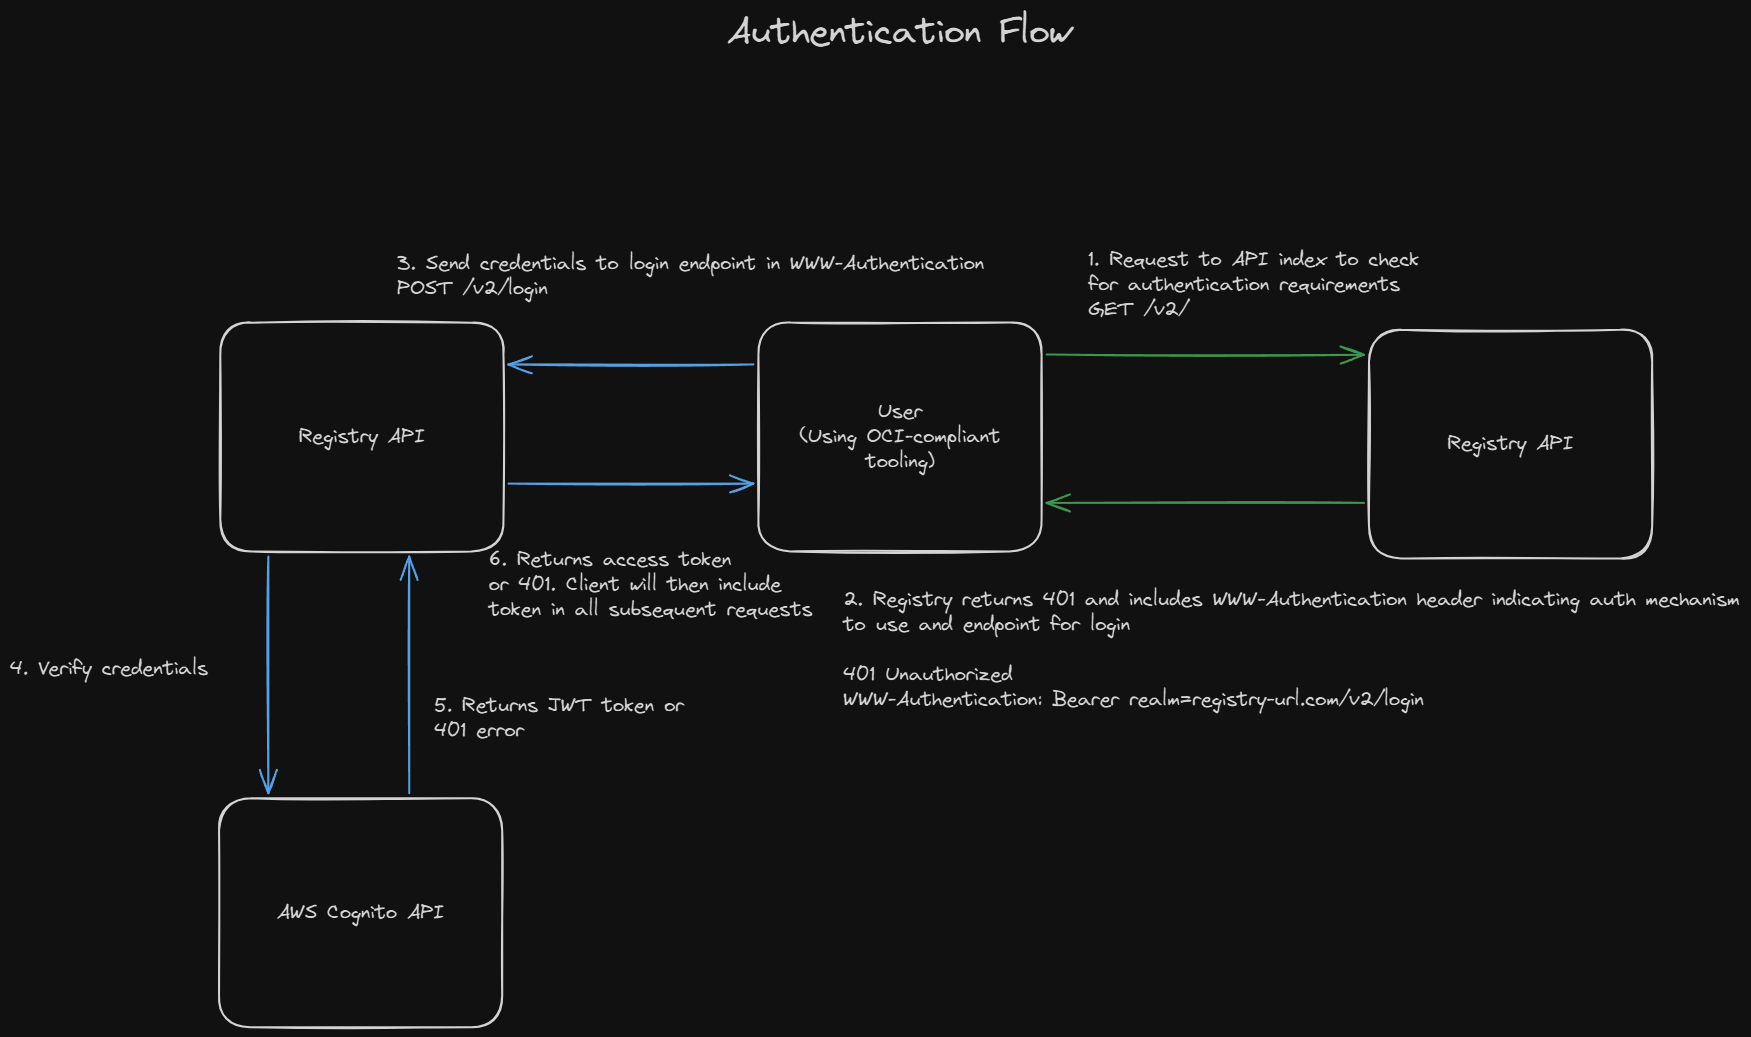
\includegraphics[scale=0.25]{appendix/auth-flow.png}

  \subsection{Appendix B. Blob Monolithic Upload with Session}
  \label{sec:appendix-b}

  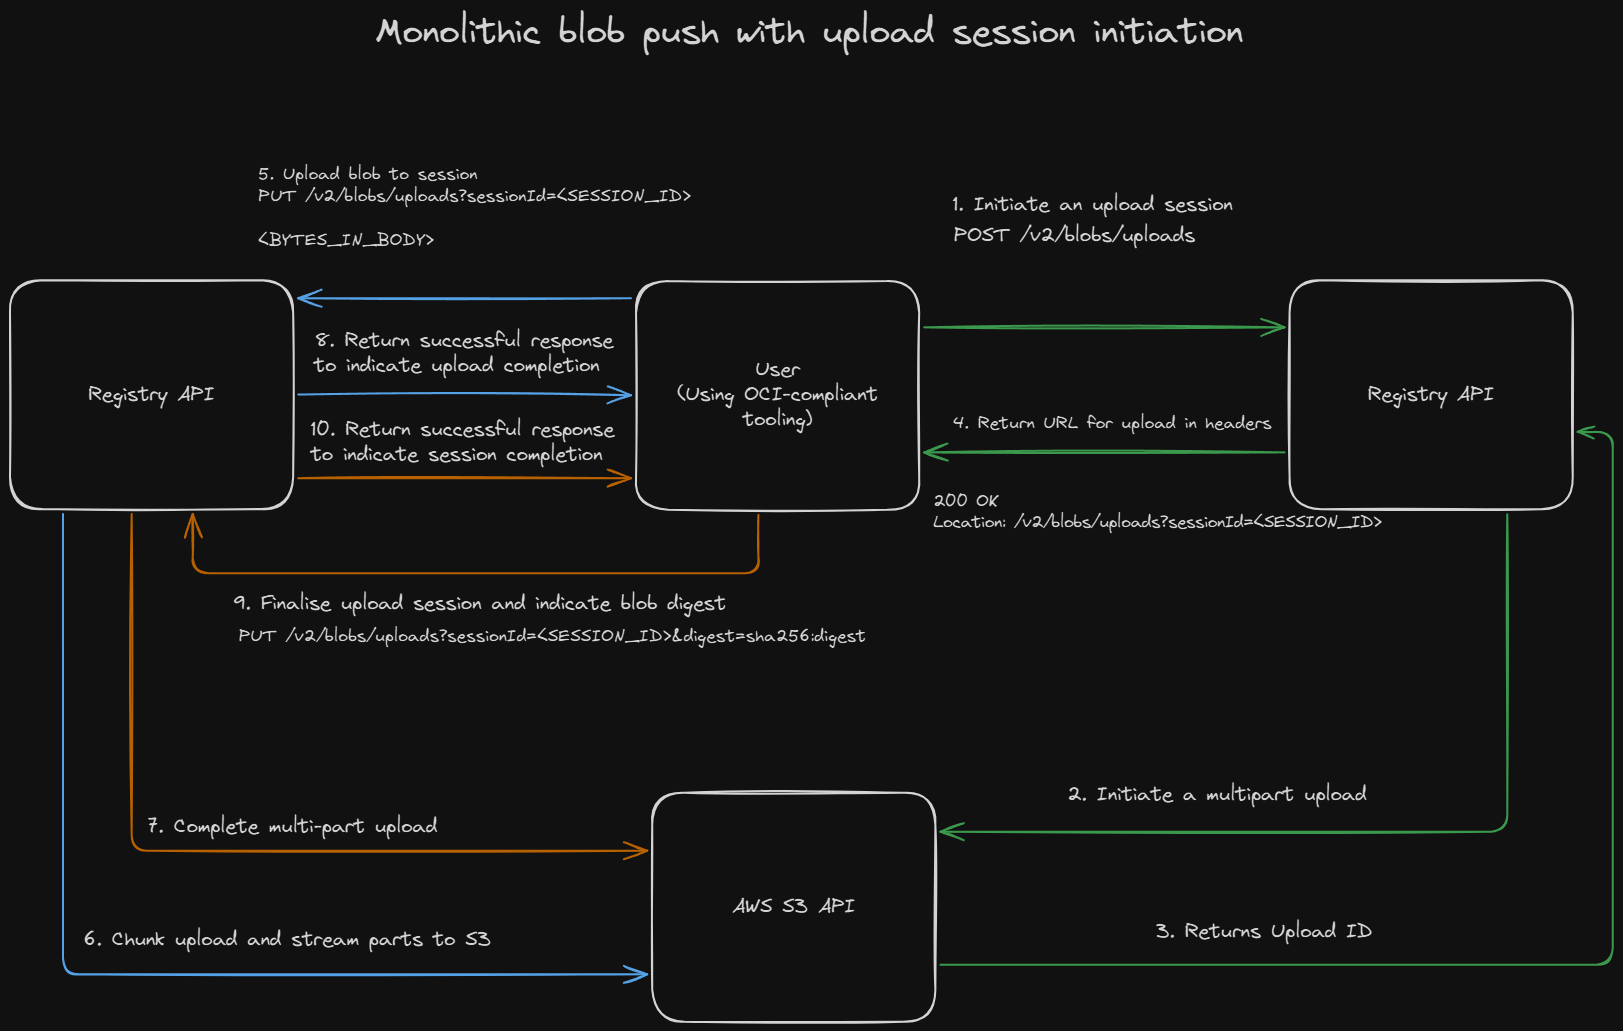
\includegraphics[scale=0.25]{appendix/blob-monolithic-upload-with-session.png}

  \subsection{Appendix C. Blob Monolithic Upload with Single POST}
  \label{sec:appendix-c}

  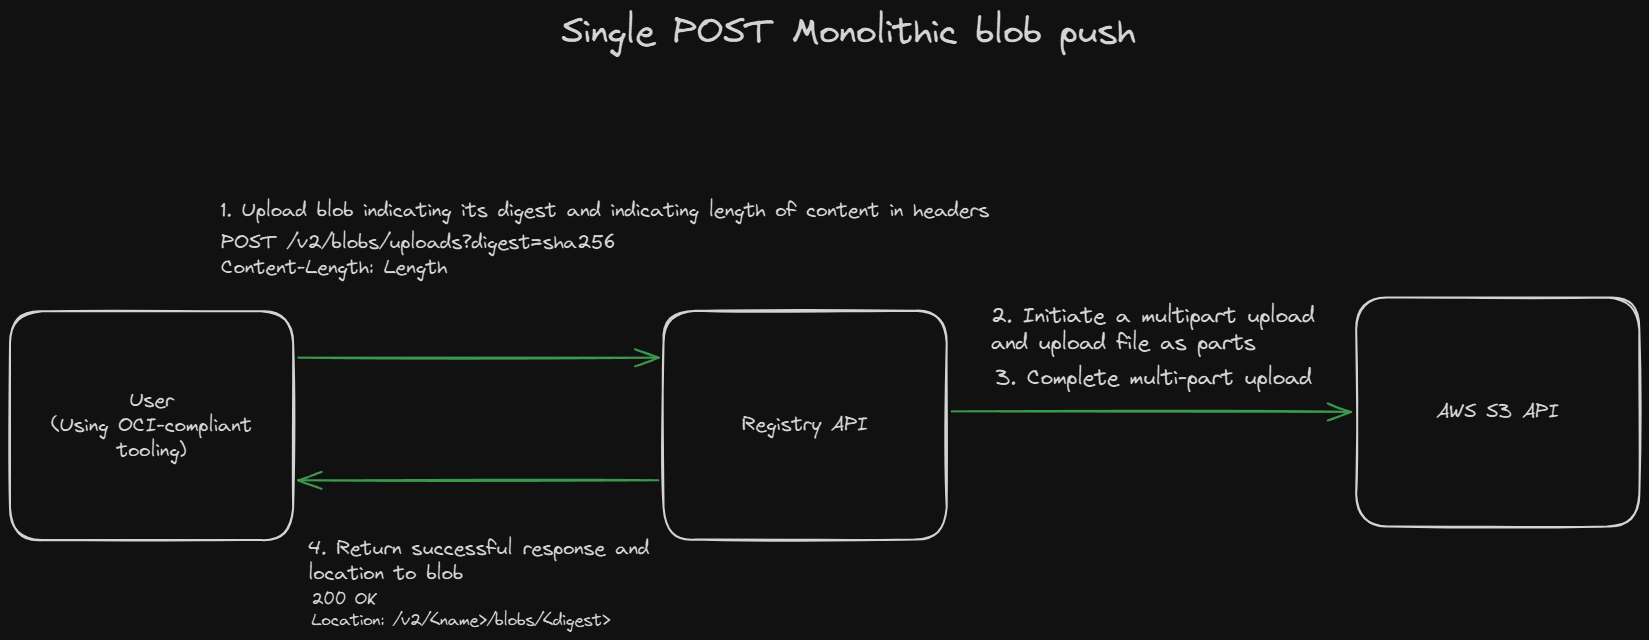
\includegraphics[scale=0.25]{appendix/blob-single-post-upload.png}

  \subsection{Appendix D. Blob Upload in Chunks}
  \label{sec:appendix-d}

  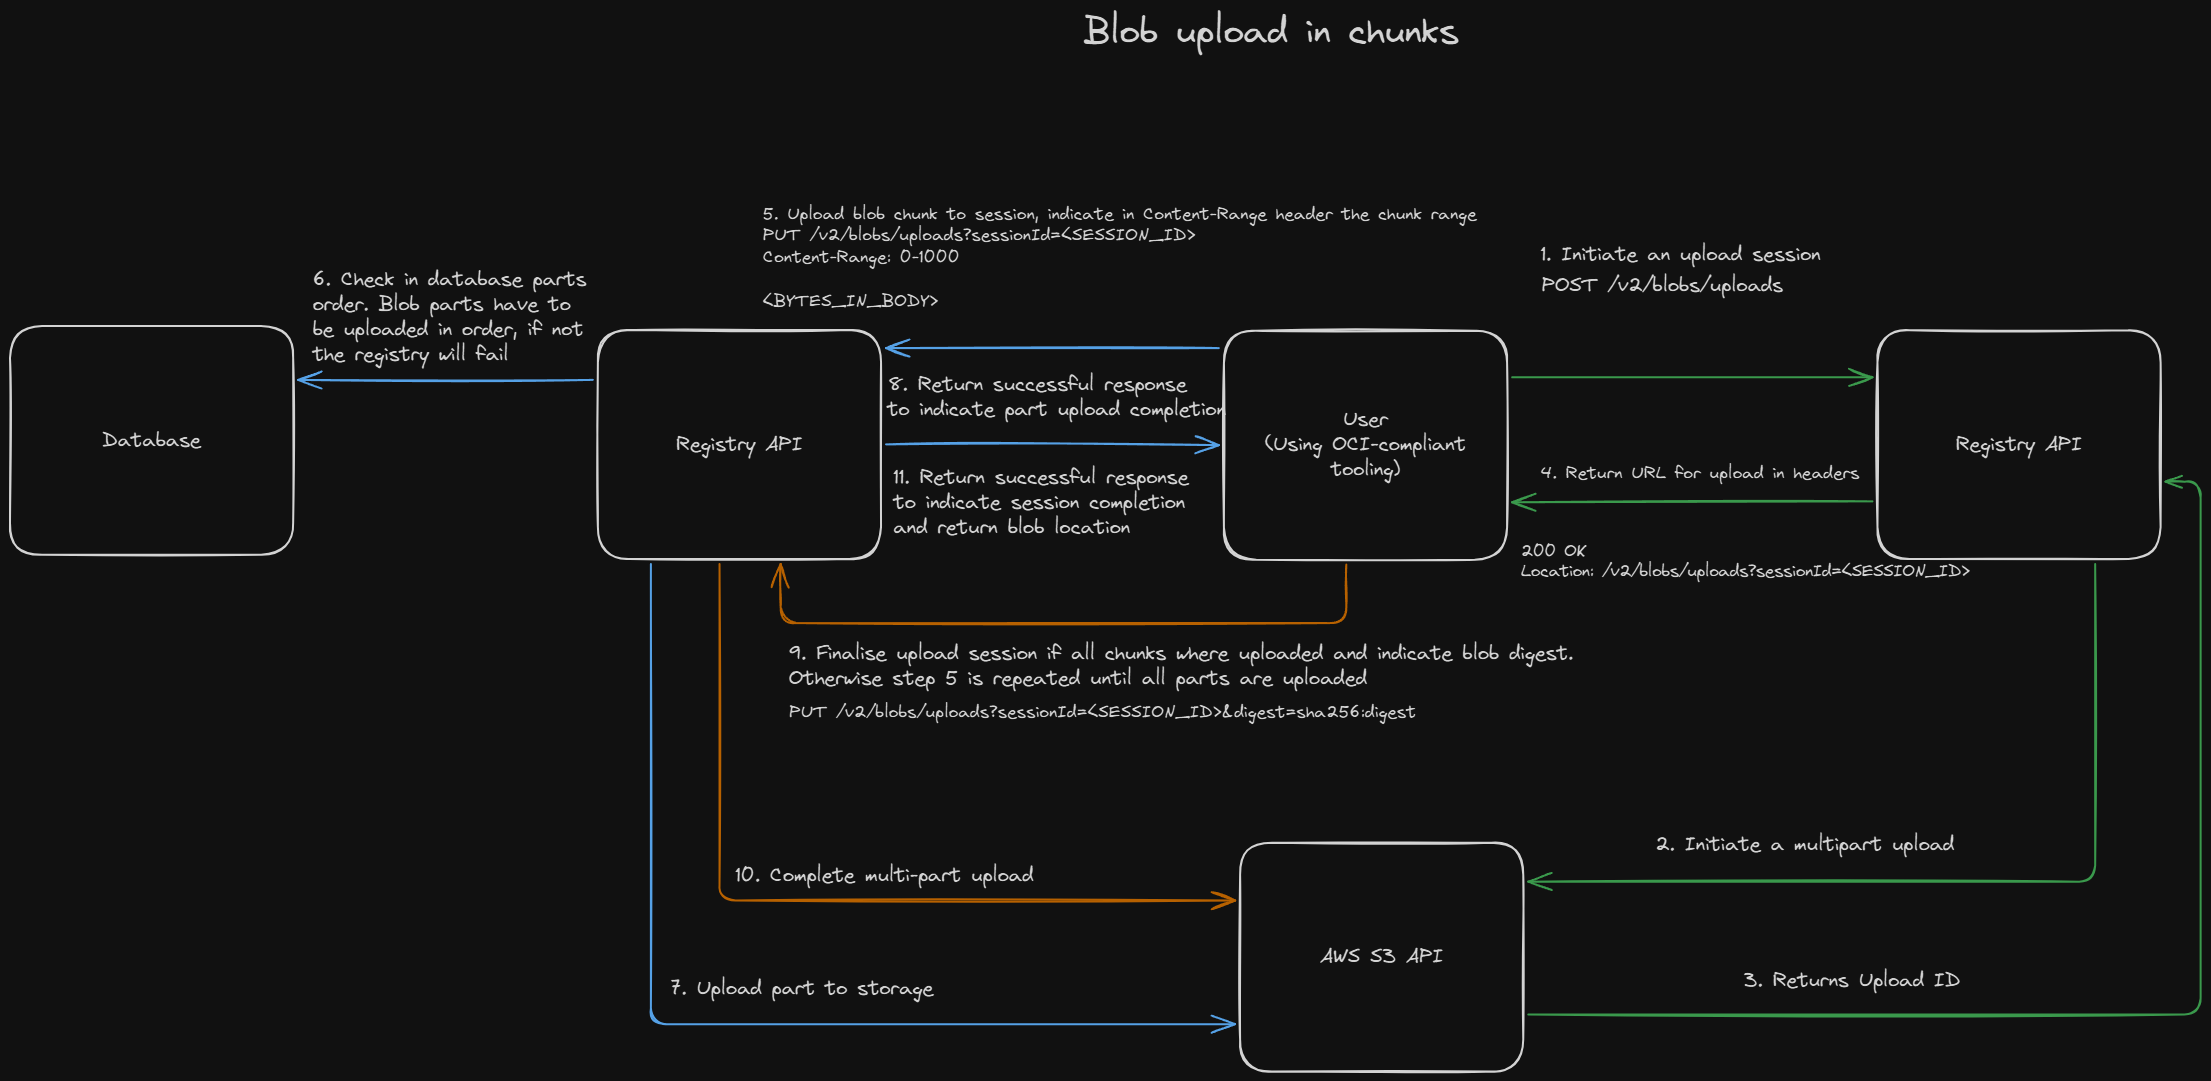
\includegraphics[scale=0.20]{appendix/blob-upload-in-chunks.png}

  \subsection{Appendix E. Download Blob}
  \label{sec:appendix-e}

  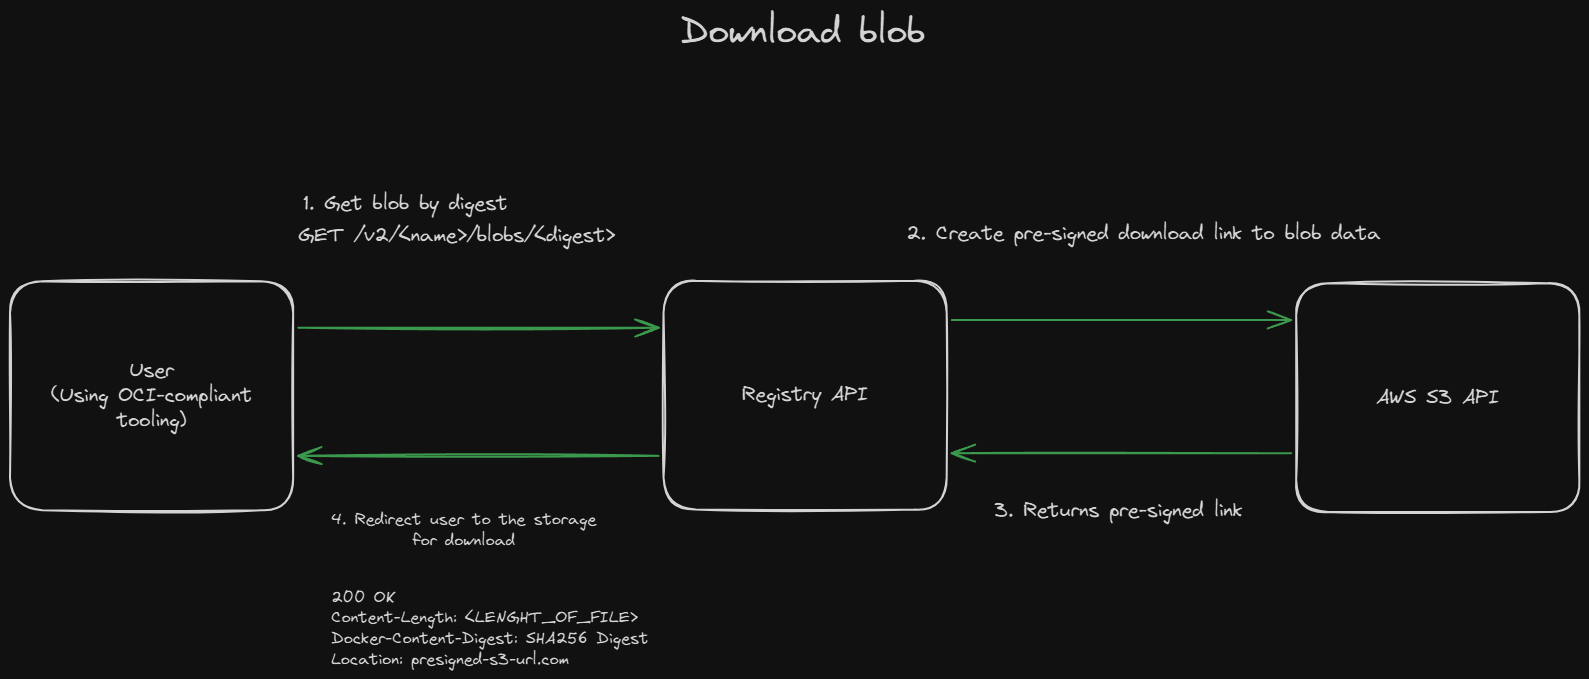
\includegraphics[scale=0.25]{appendix/download-blob.png}

  \subsection{Appendix F. Python Upload Flow}
  \label{sec:appendix-f}

  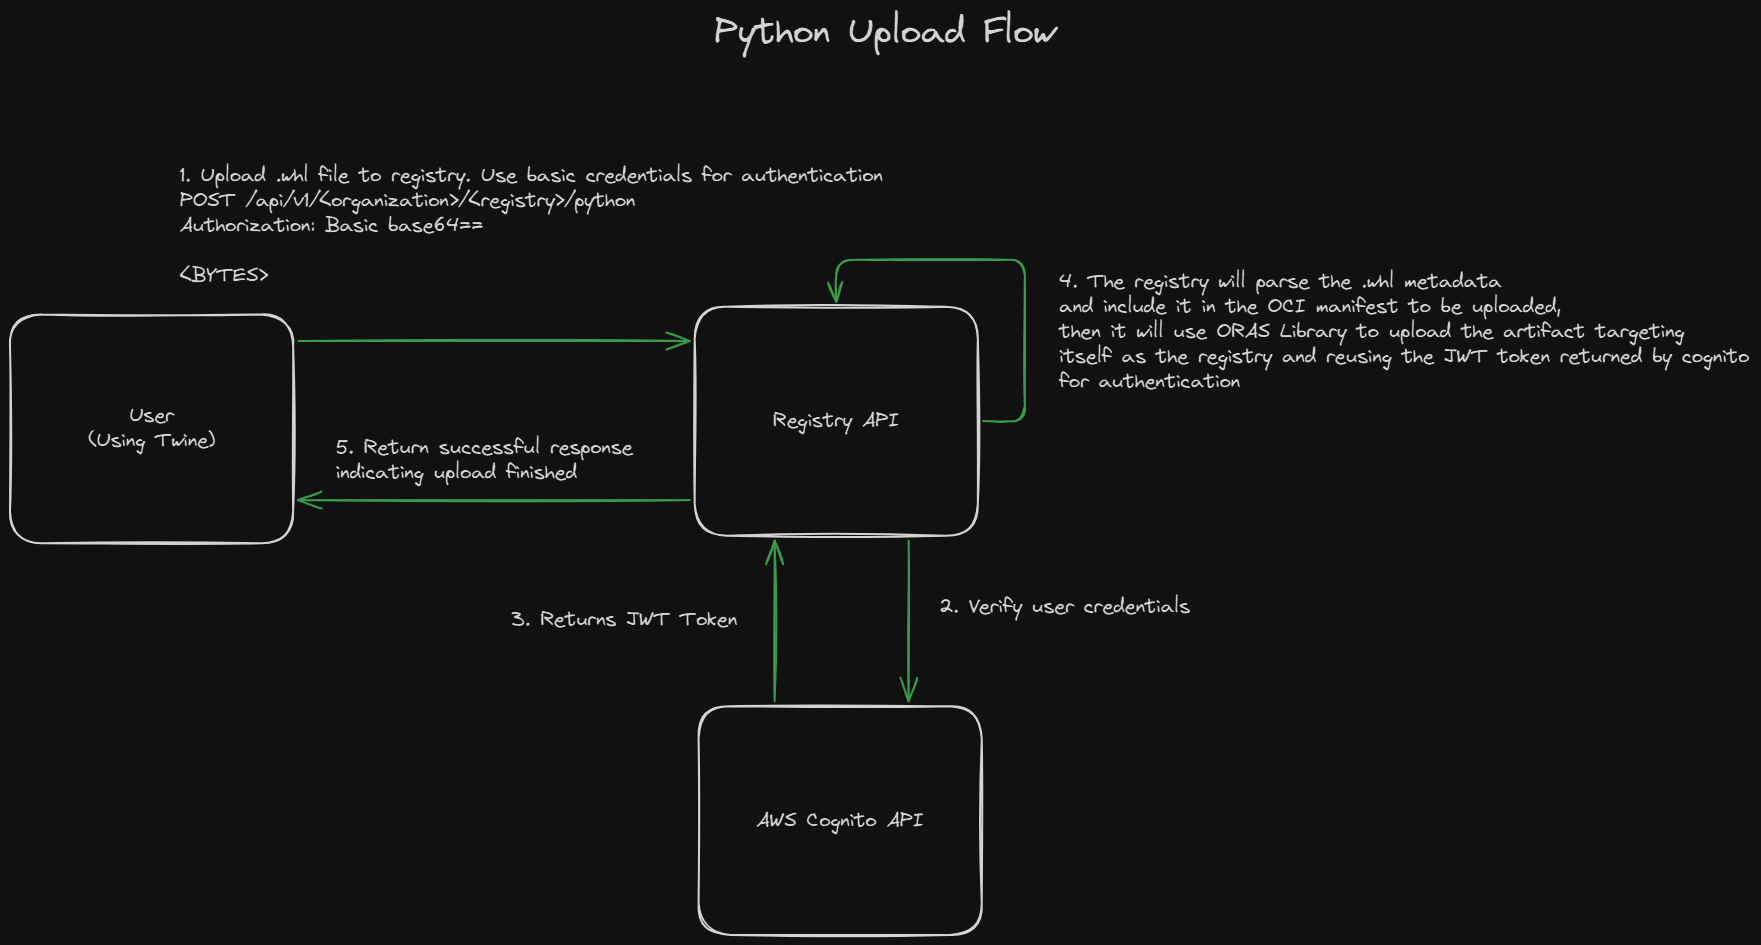
\includegraphics[scale=0.25]{appendix/python-upload-flow.png}

  \subsection{Appendix G. Python OCI Manifest}
  \label{sec:appendix-g}

  \verbatiminput{./images/appendix/python-package-manifest.json}

  \subsection{Appendix H. Python Simple Repository Index}
  \label{sec:appendix-h}

  \verbatiminput{./images/appendix/simple-repository-index.html}

  \subsection{Appendix I. Python Simple Repository Index - List Versions}
  \label{sec:appendix-i}

  \verbatiminput{./images/appendix/simple-repository-index-2.html}

  \subsection{Appendix J. Example of Database Repository}
  \label{sec:appendix-j}

  \begin{lstlisting}[language=Golang]
    package repositories

    import (
      "context"

      "repositories/ent"
      "repositories/ent/organization"
      "repositories/ent/user"
    )

    type OrganizationRepository struct {
      dbClient *ent.Client
    }

    func NewOrganizationRepository(dbClient *ent.Client) *OrganizationRepository {
      return &OrganizationRepository{
        dbClient: dbClient,
      }
    }

    func (orgRepo *OrganizationRepository) GetForUser(ctx context.Context, sub string) ([]*ent.Organization, error) {
      return orgRepo.dbClient.Organization.Query().Where(
        organization.HasMembersWith(
          user.Sub(sub),
        ),
      ).All(ctx)
    }
  \end{lstlisting}

  \subsection{Appendix K. Example of Handler}
  \label{sec:appendix-k}

  \begin{lstlisting}[language=Golang]
    package api

    import (
      "encoding/json"
      "log"
      "net/http"

      "pkg/config"
      "pkg/repositories"
      "github.com/go-chi/chi/v5"
    )

    type OrganizationsHandler struct {
      Config                 *config.AppConfig
      OrganizationRepository *repositories.OrganizationRepository
    }

    func (oh *OrganizationsHandler) GetOrganizationsForUser(w http.ResponseWriter, r *http.Request) {
      // Get user SUB ID from the context. This value is added to the context by middleware
      userSub := r.Context().Value("user_sub").(string)

      // Query the database for all the organizations the user belongs to
      orgs, err := oh.OrganizationRepository.GetForUser(r.Context(), userSub)
      if err != nil {
        log.Println(err)
        w.WriteHeader(500)
        return
      }

      // Return a JSON response with all the orgs the user is a part of
      w.WriteHeader(http.StatusOK)
      json.NewEncoder(w).Encode(orgs)
    }

  \end{lstlisting}

  \subsection{Appendix L. Middleware Flow}
  \label{sec:appendix-l}

  {\parindent0pt
    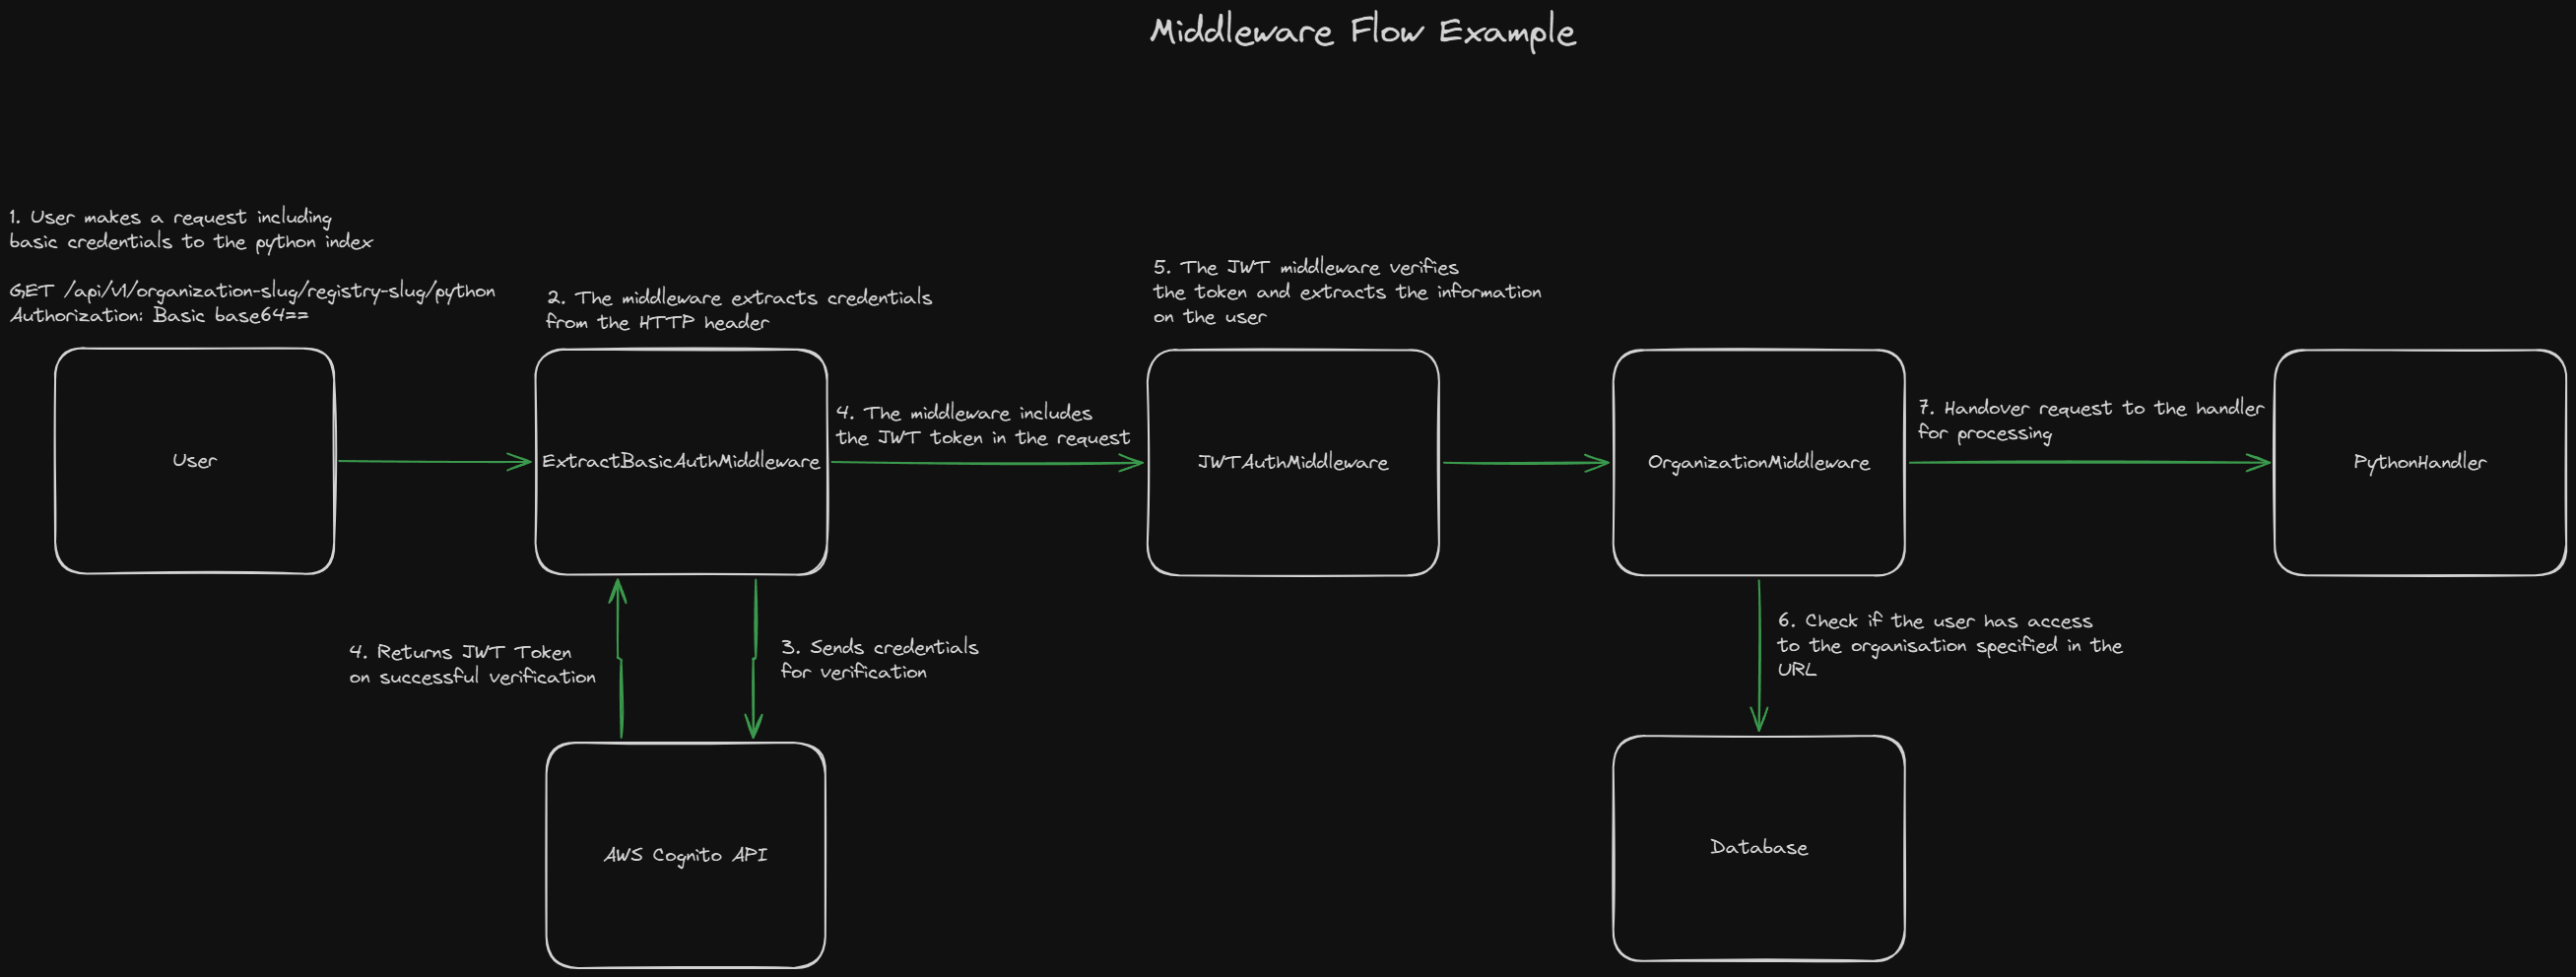
\includegraphics[scale=0.18]{appendix/middleware-flow-python-example.png}
  }

  \subsection{Appendix M. Web UI Screenshots}
  \label{sec:appendix-m}

  \subsubsection{Login and signup}

  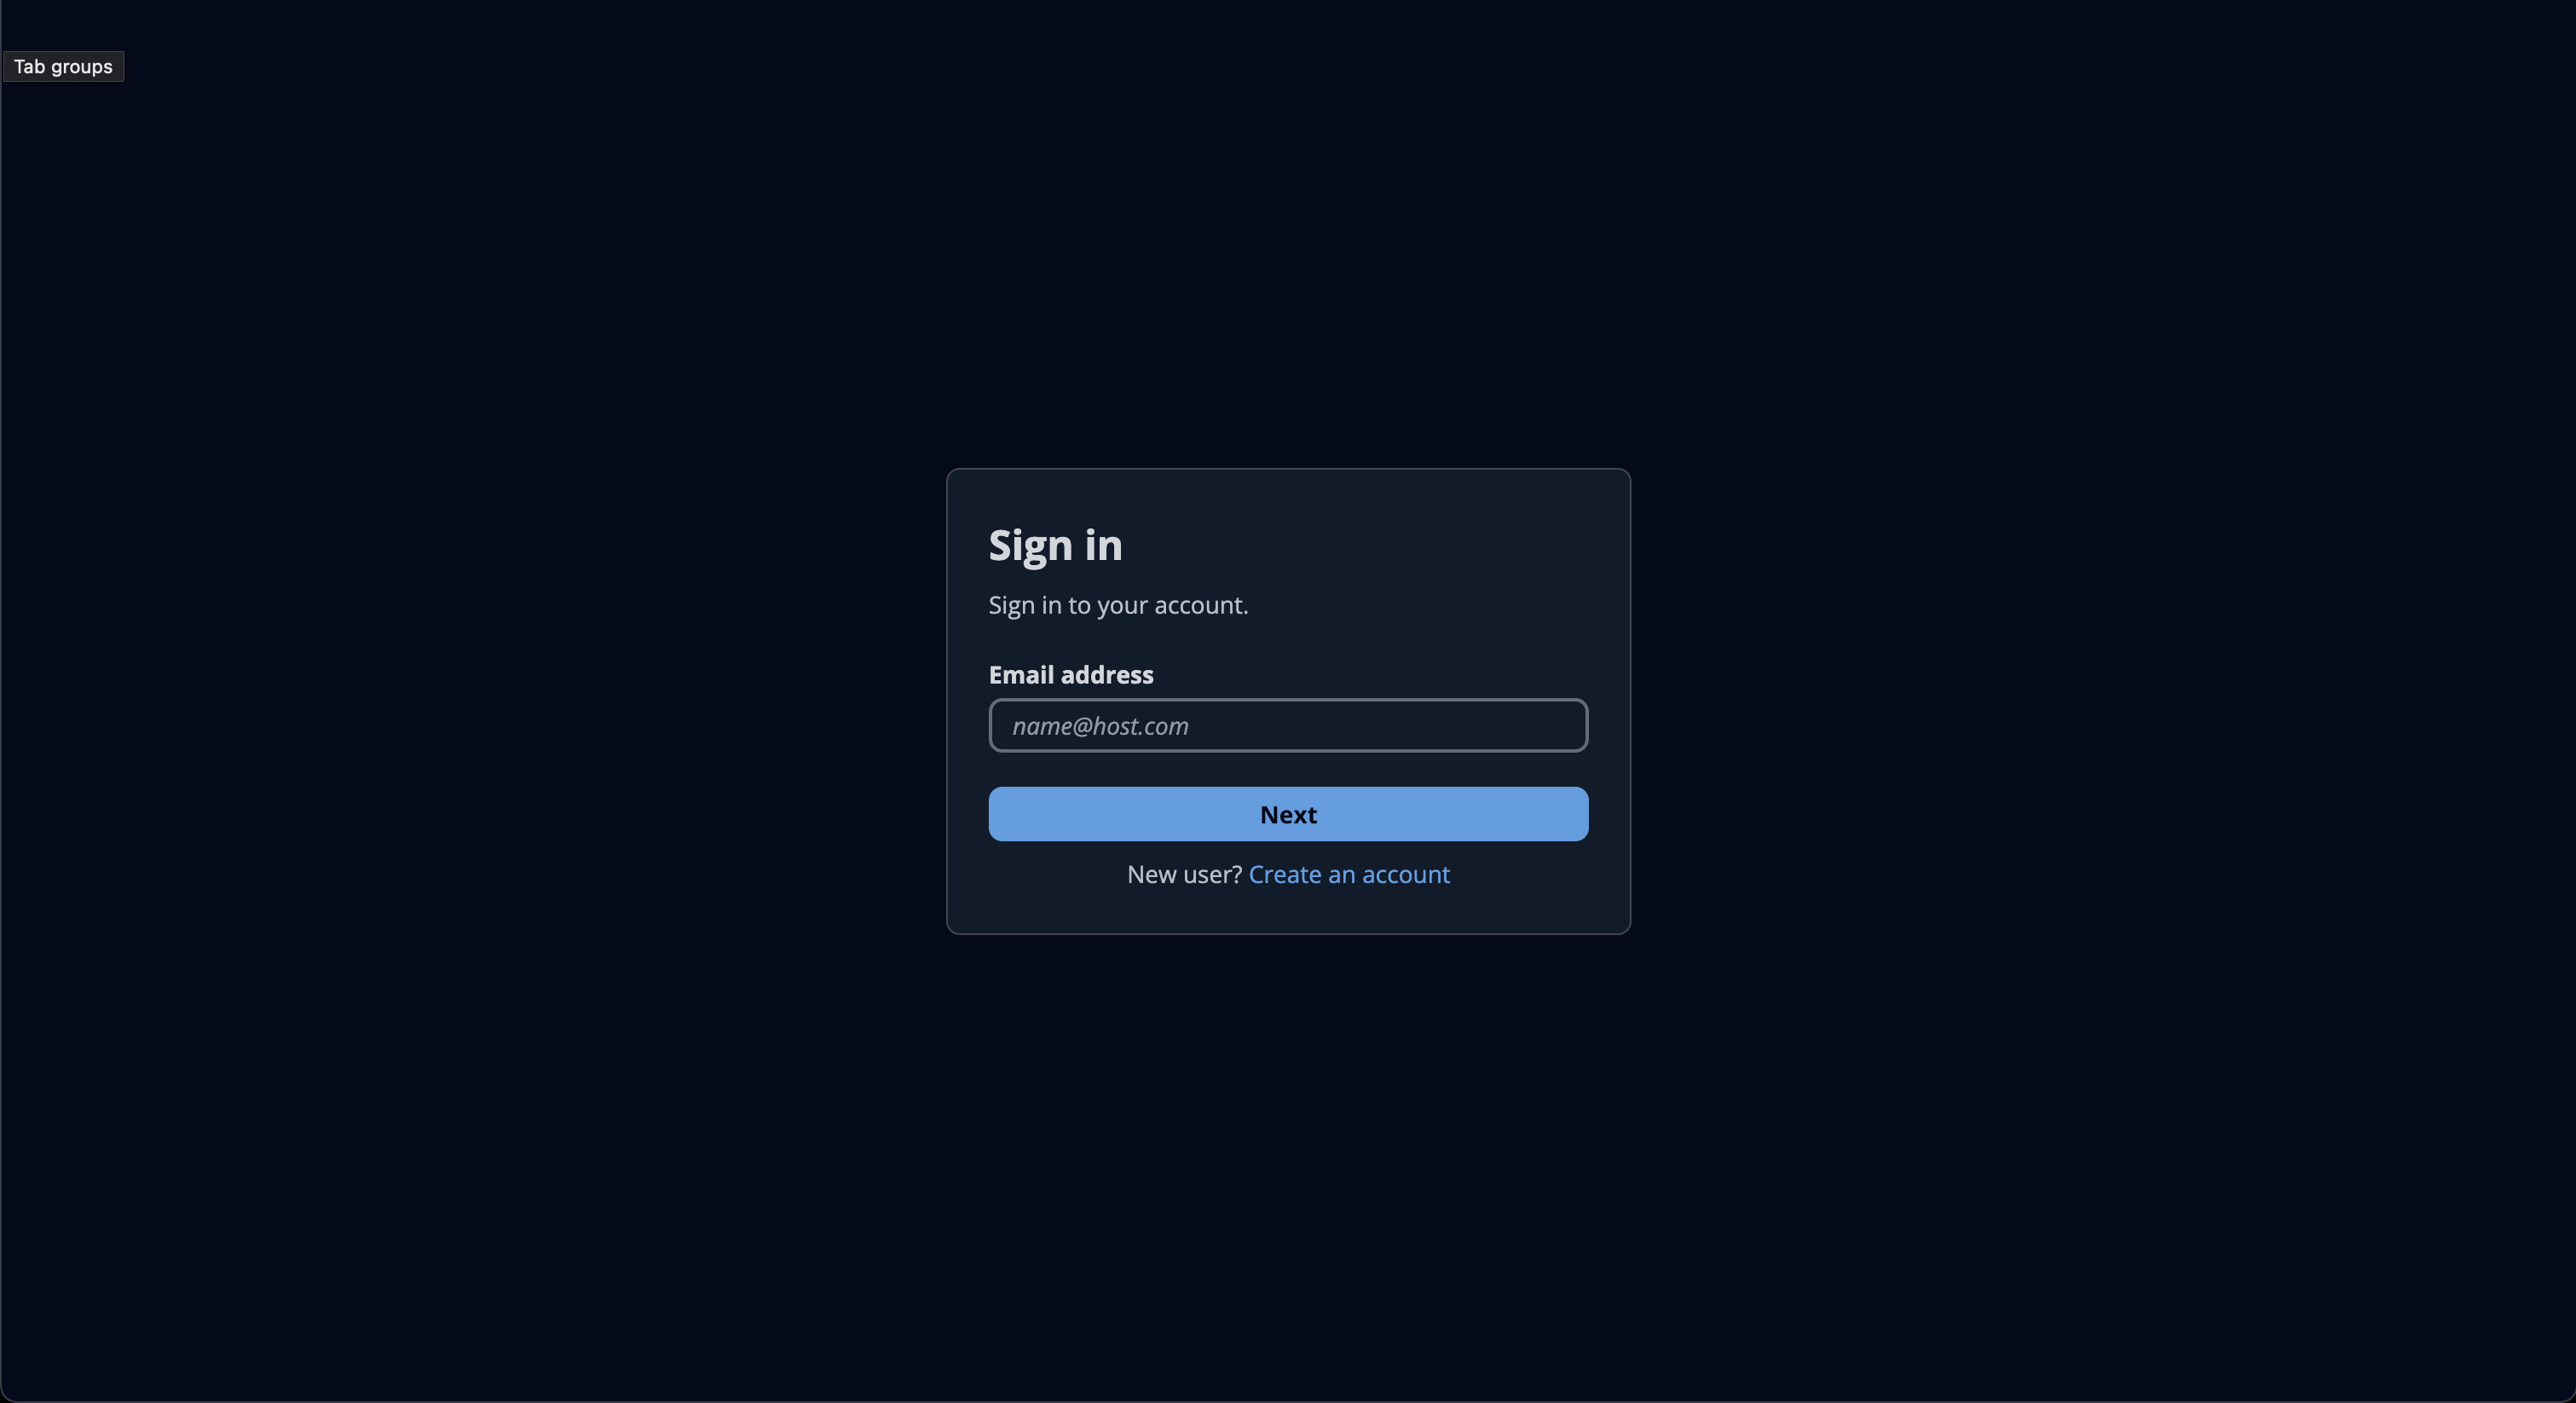
\includegraphics[scale=0.28]{screenshots/signin.png}

  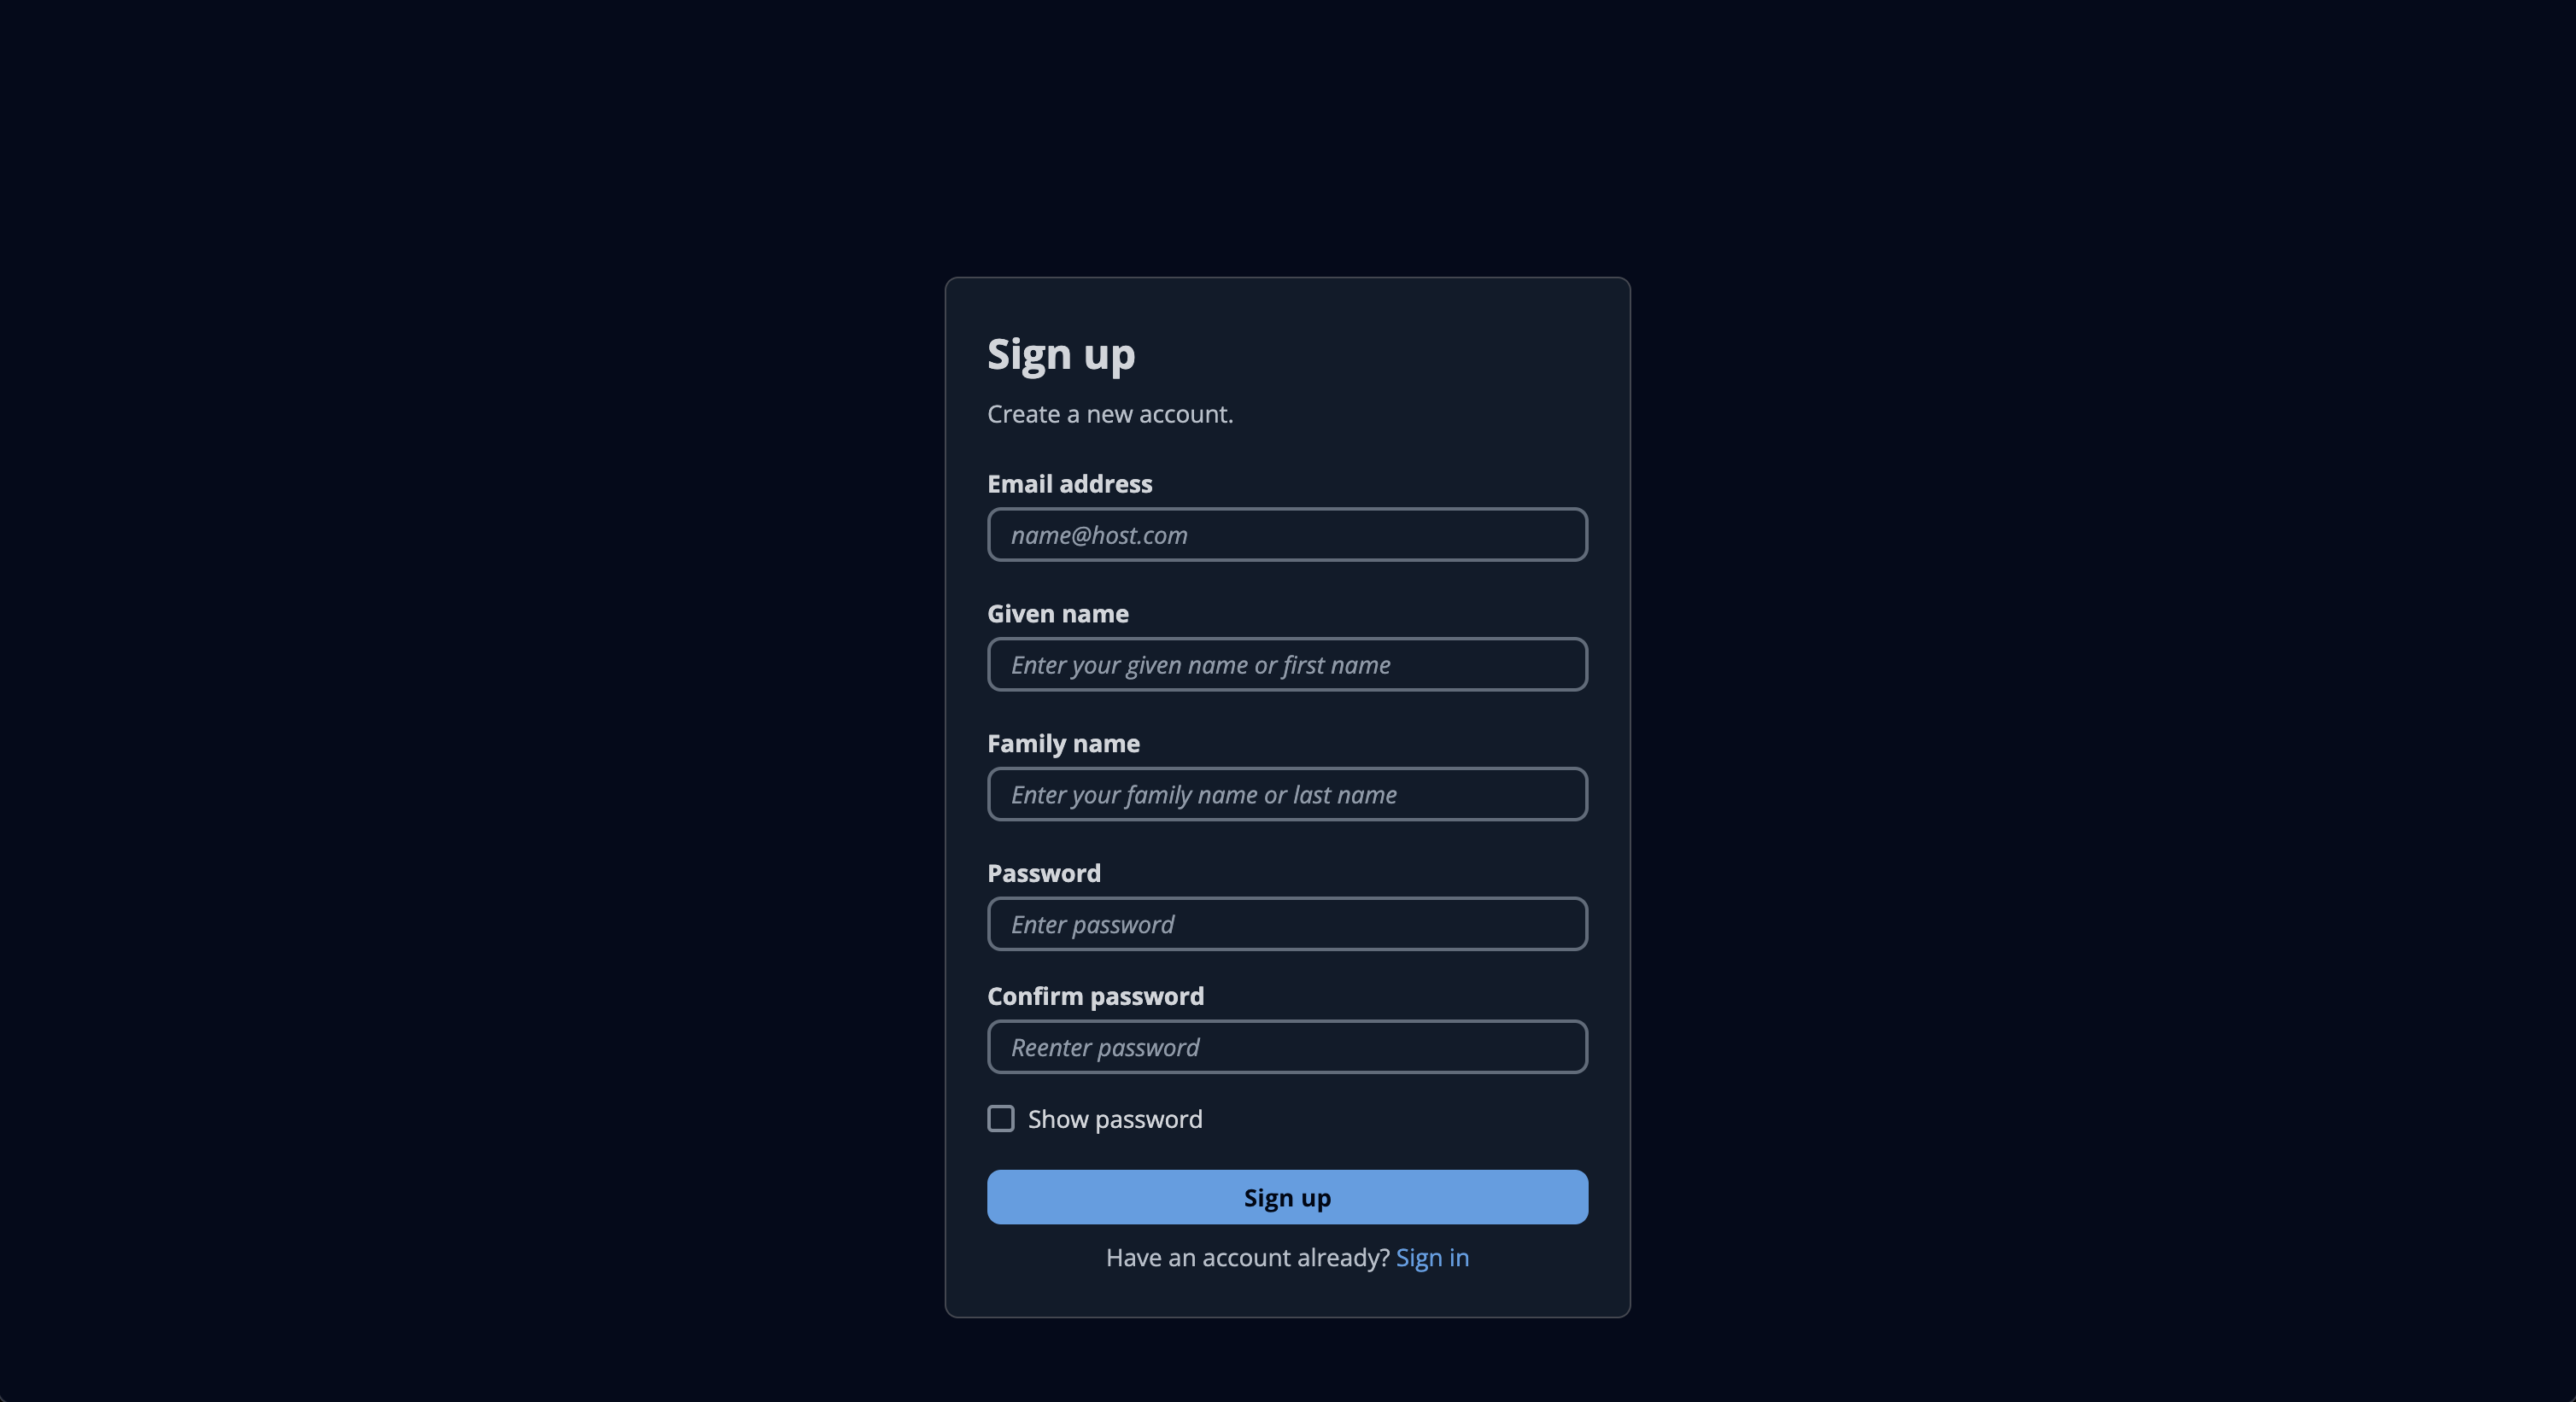
\includegraphics[scale=0.28]{screenshots/signup.png}

  \subsubsection{Dashboard}

  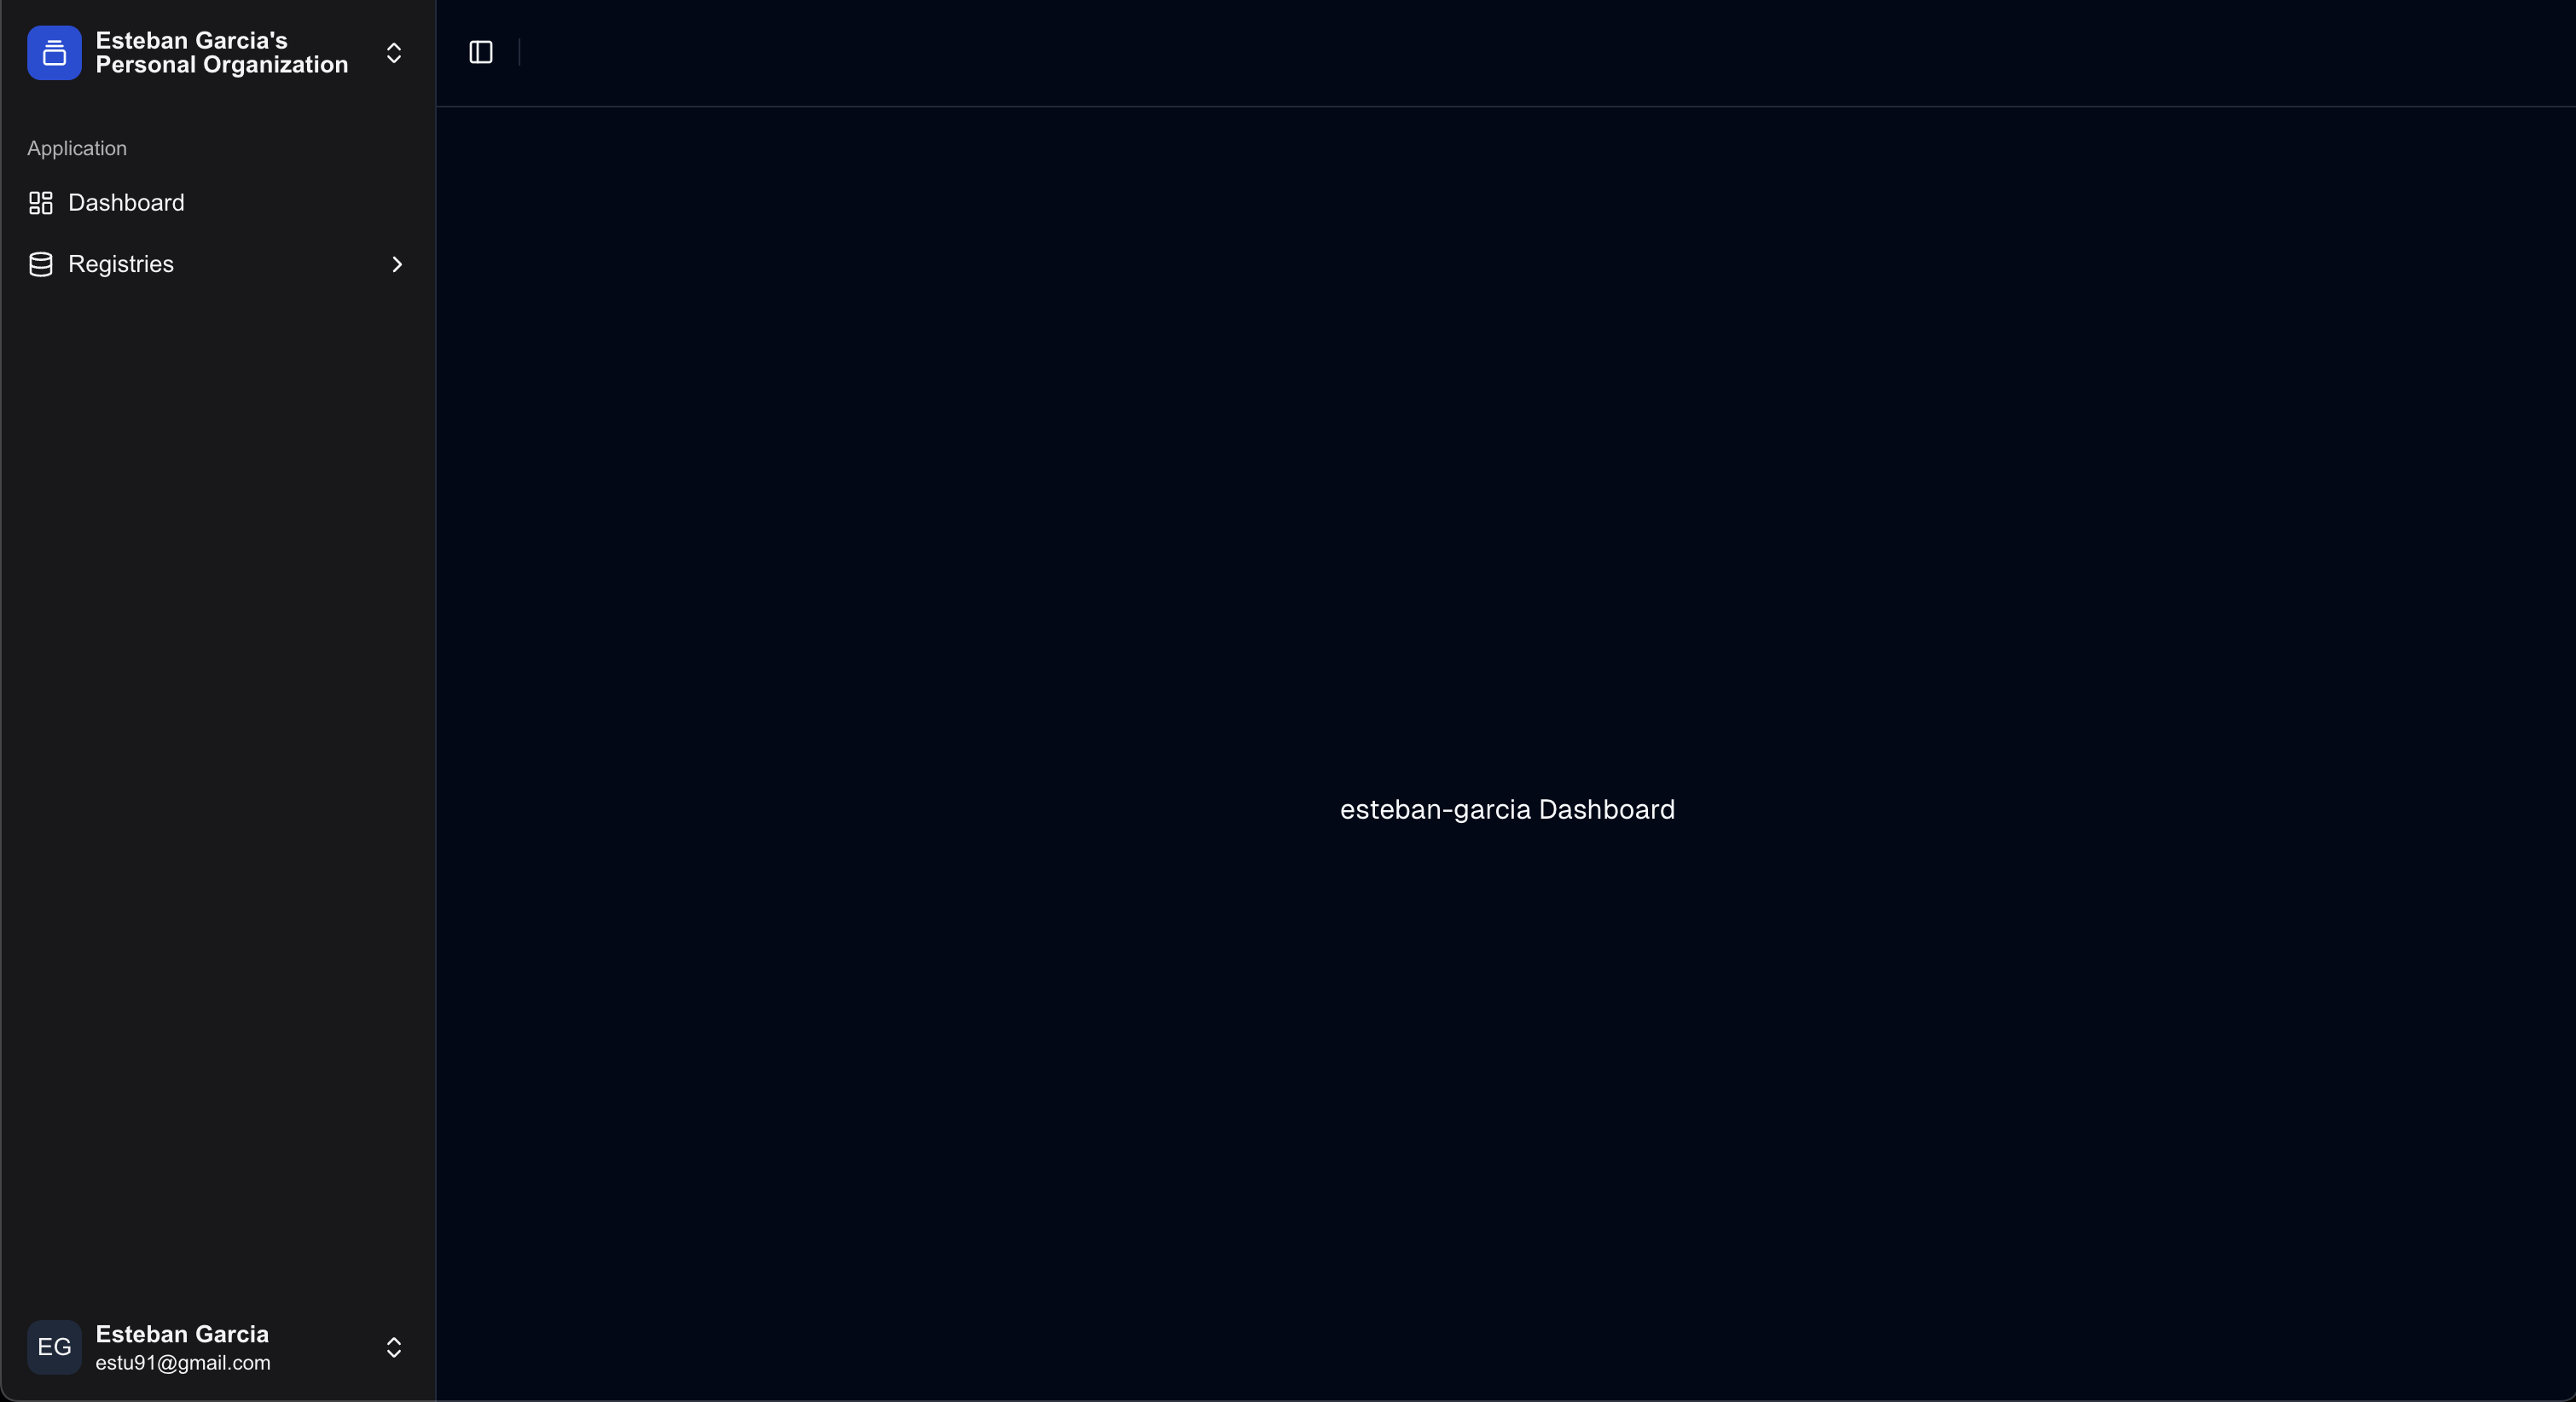
\includegraphics[scale=0.28]{screenshots/dashboard.png} 

  \subsubsection{Registries}

  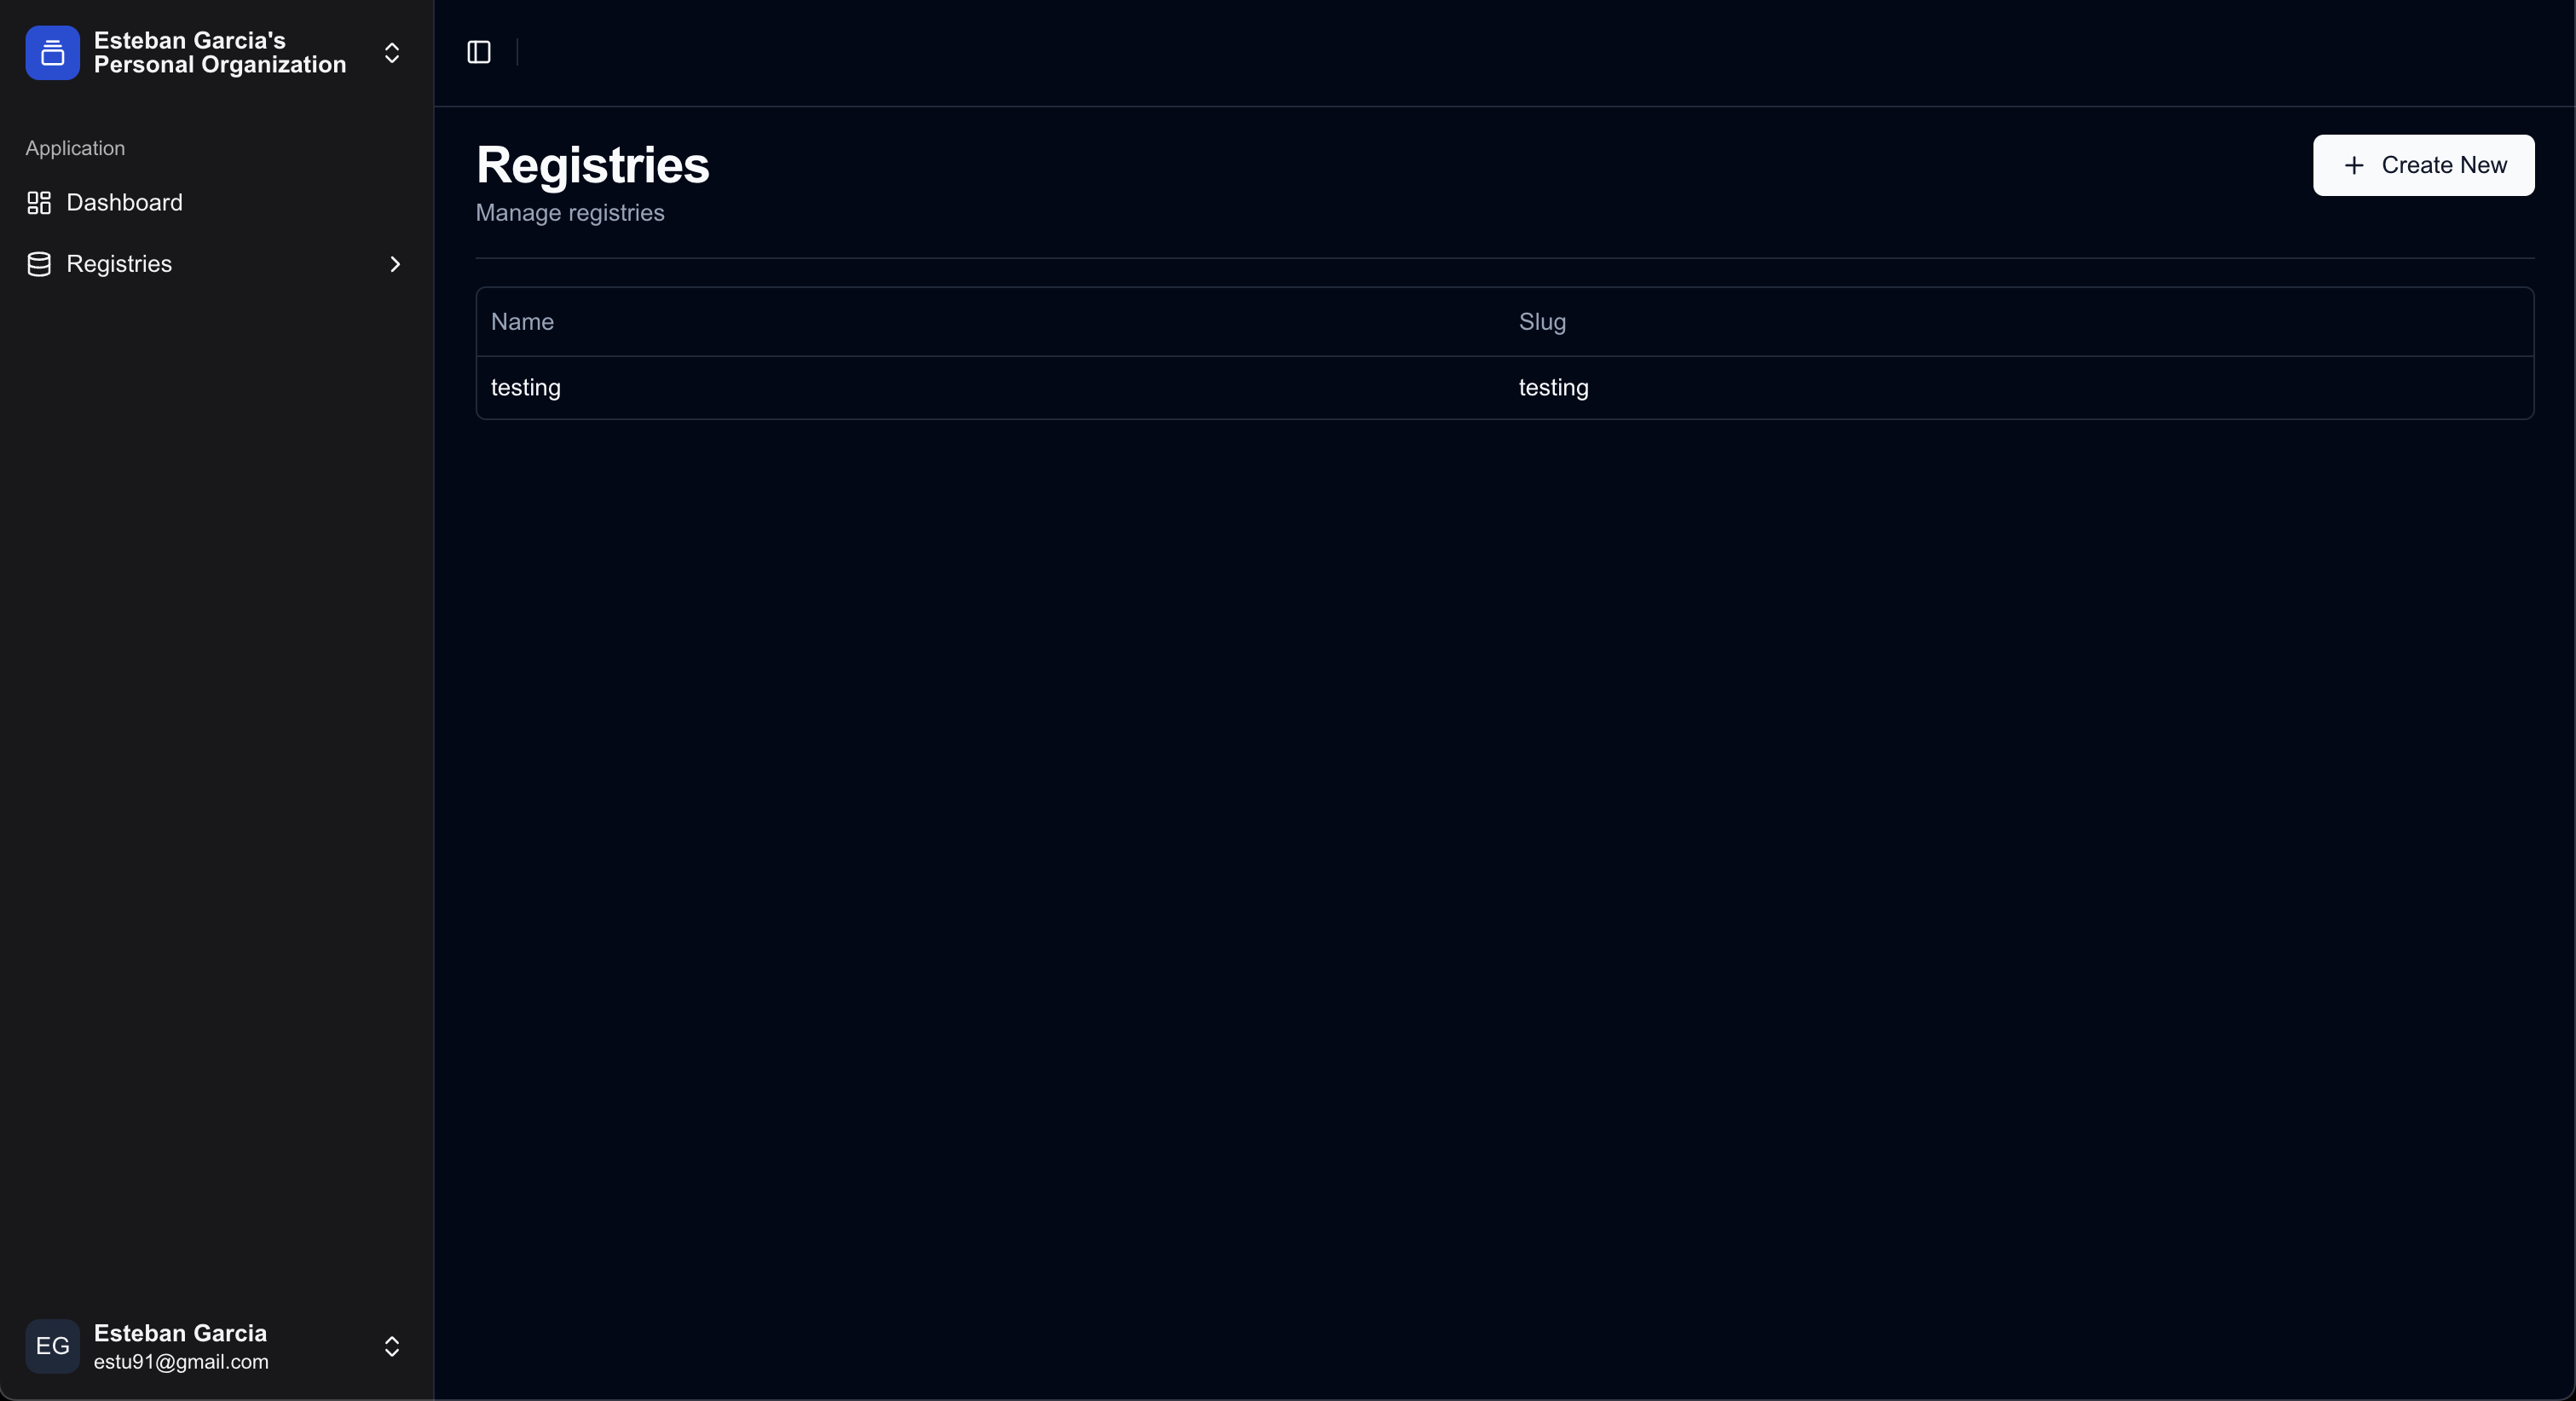
\includegraphics[scale=0.28]{screenshots/registries.png}

  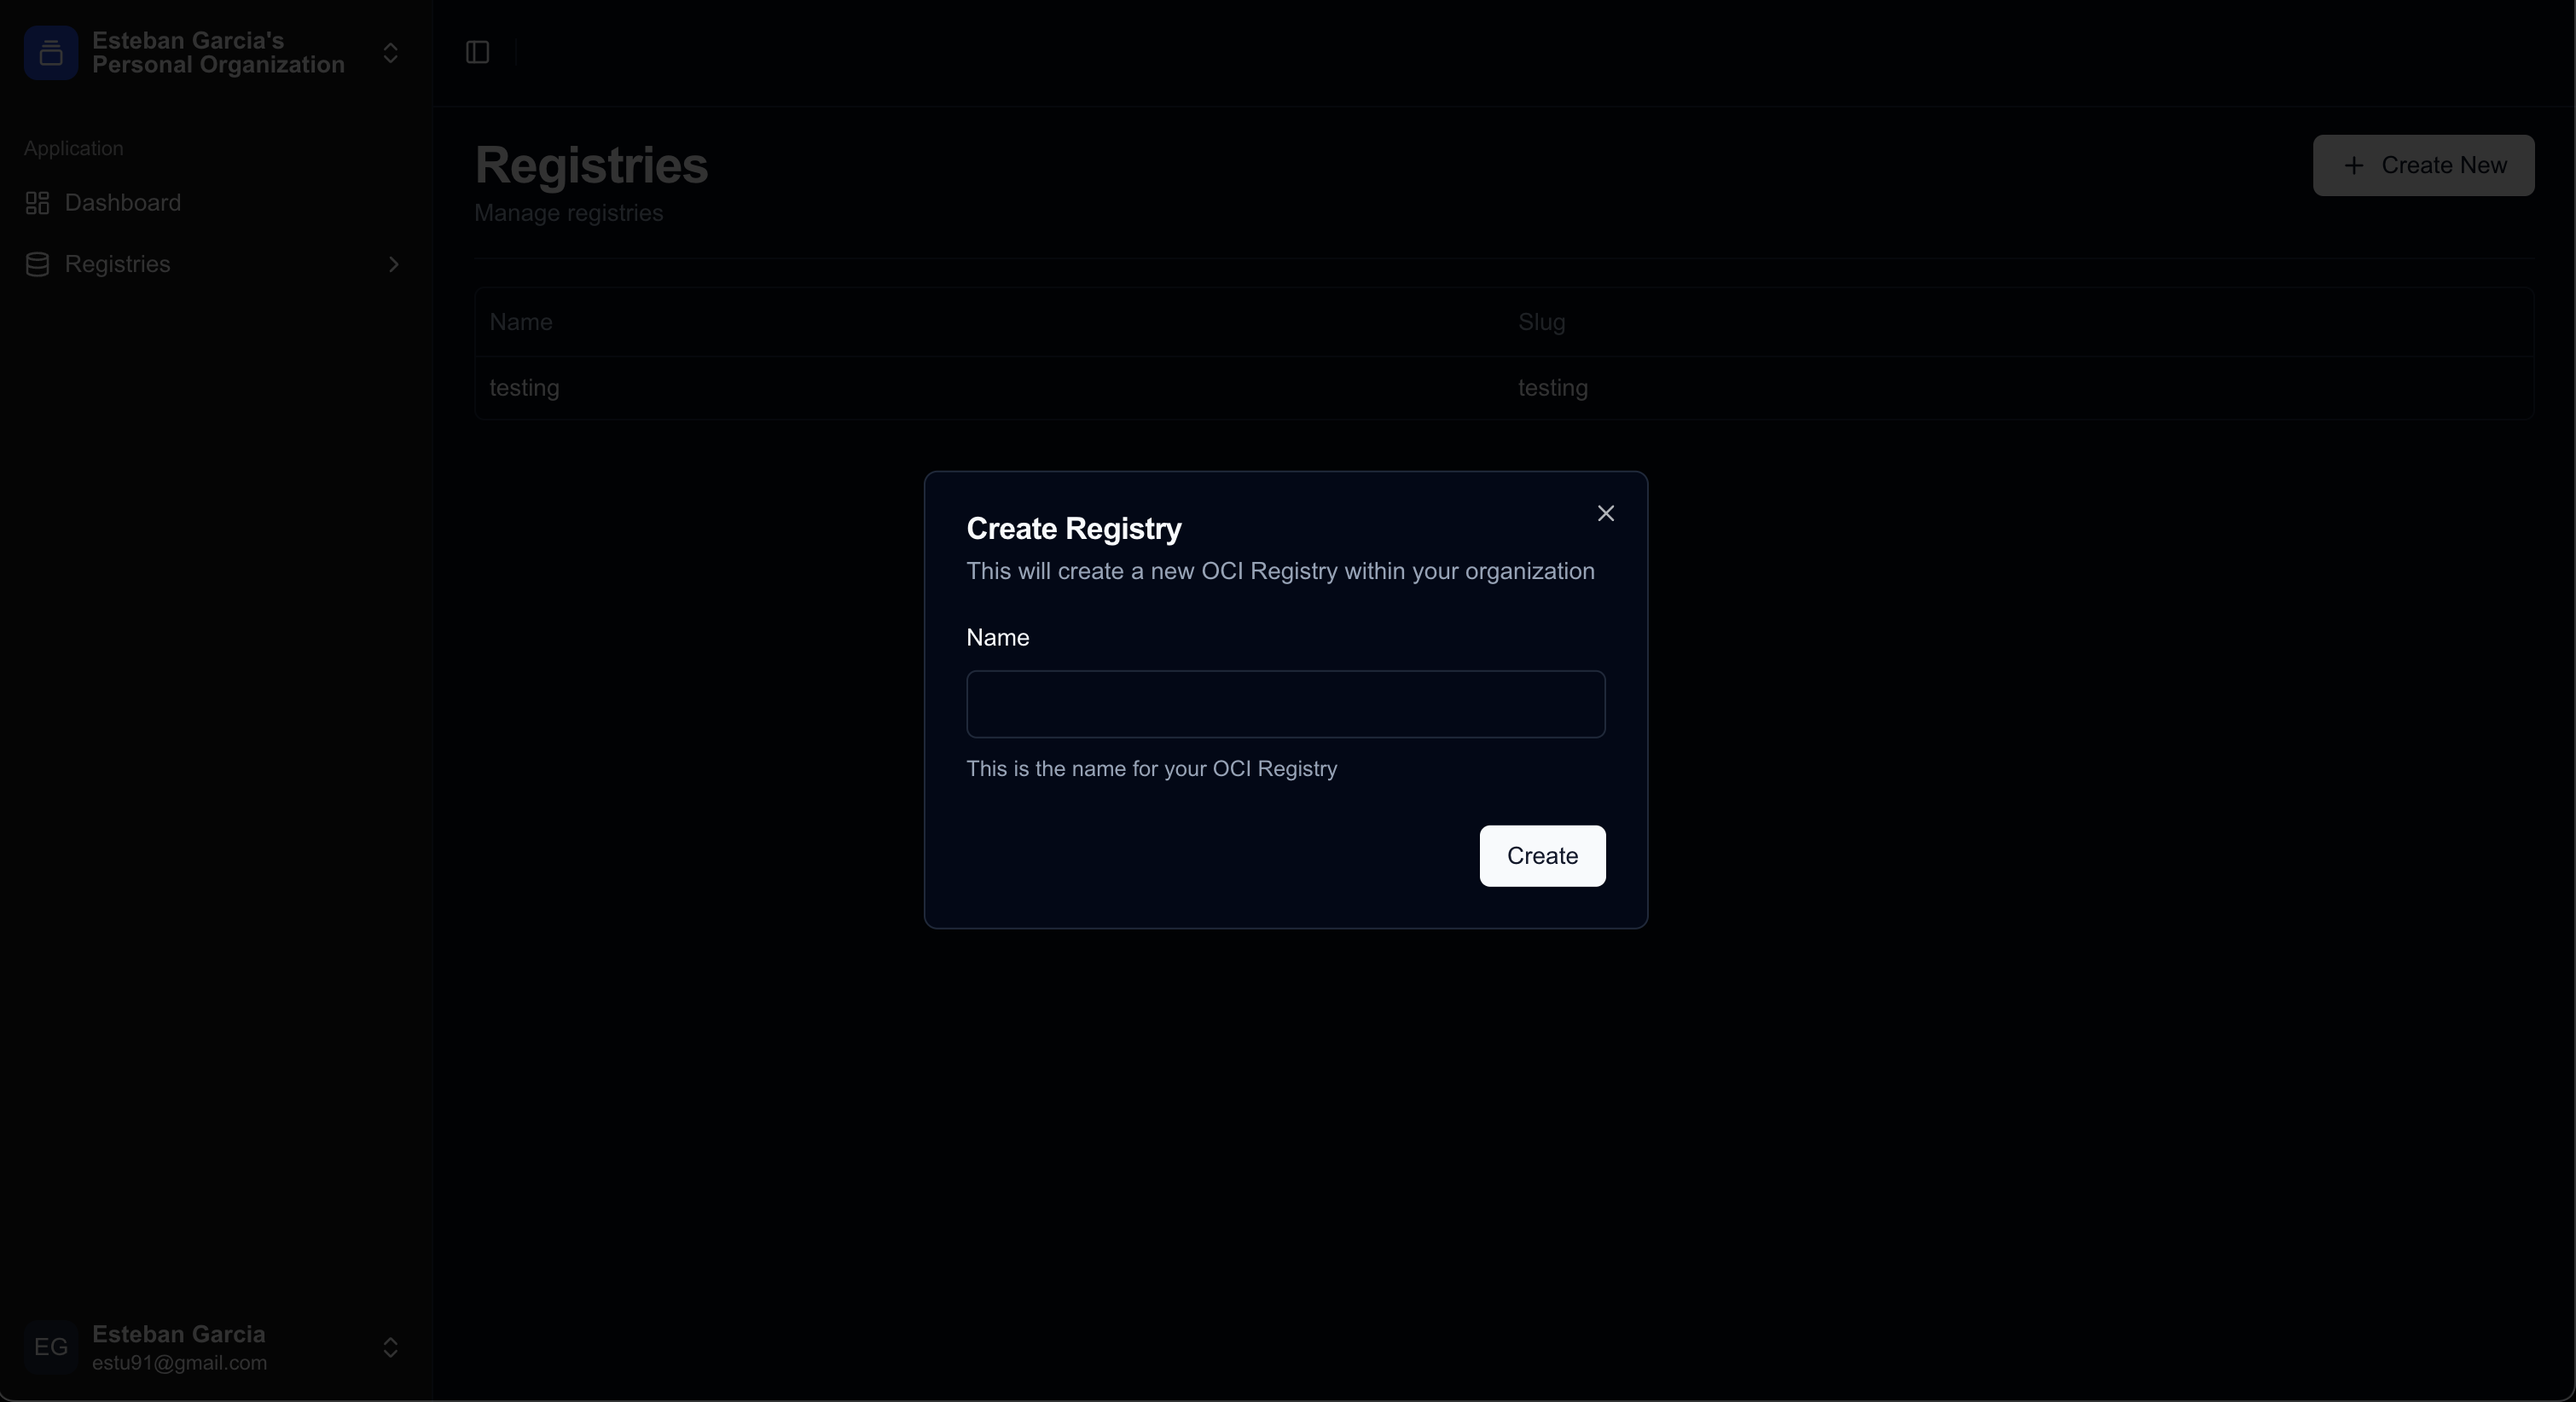
\includegraphics[scale=0.28]{screenshots/create-registry.png}

  \subsubsection{Repositories}

  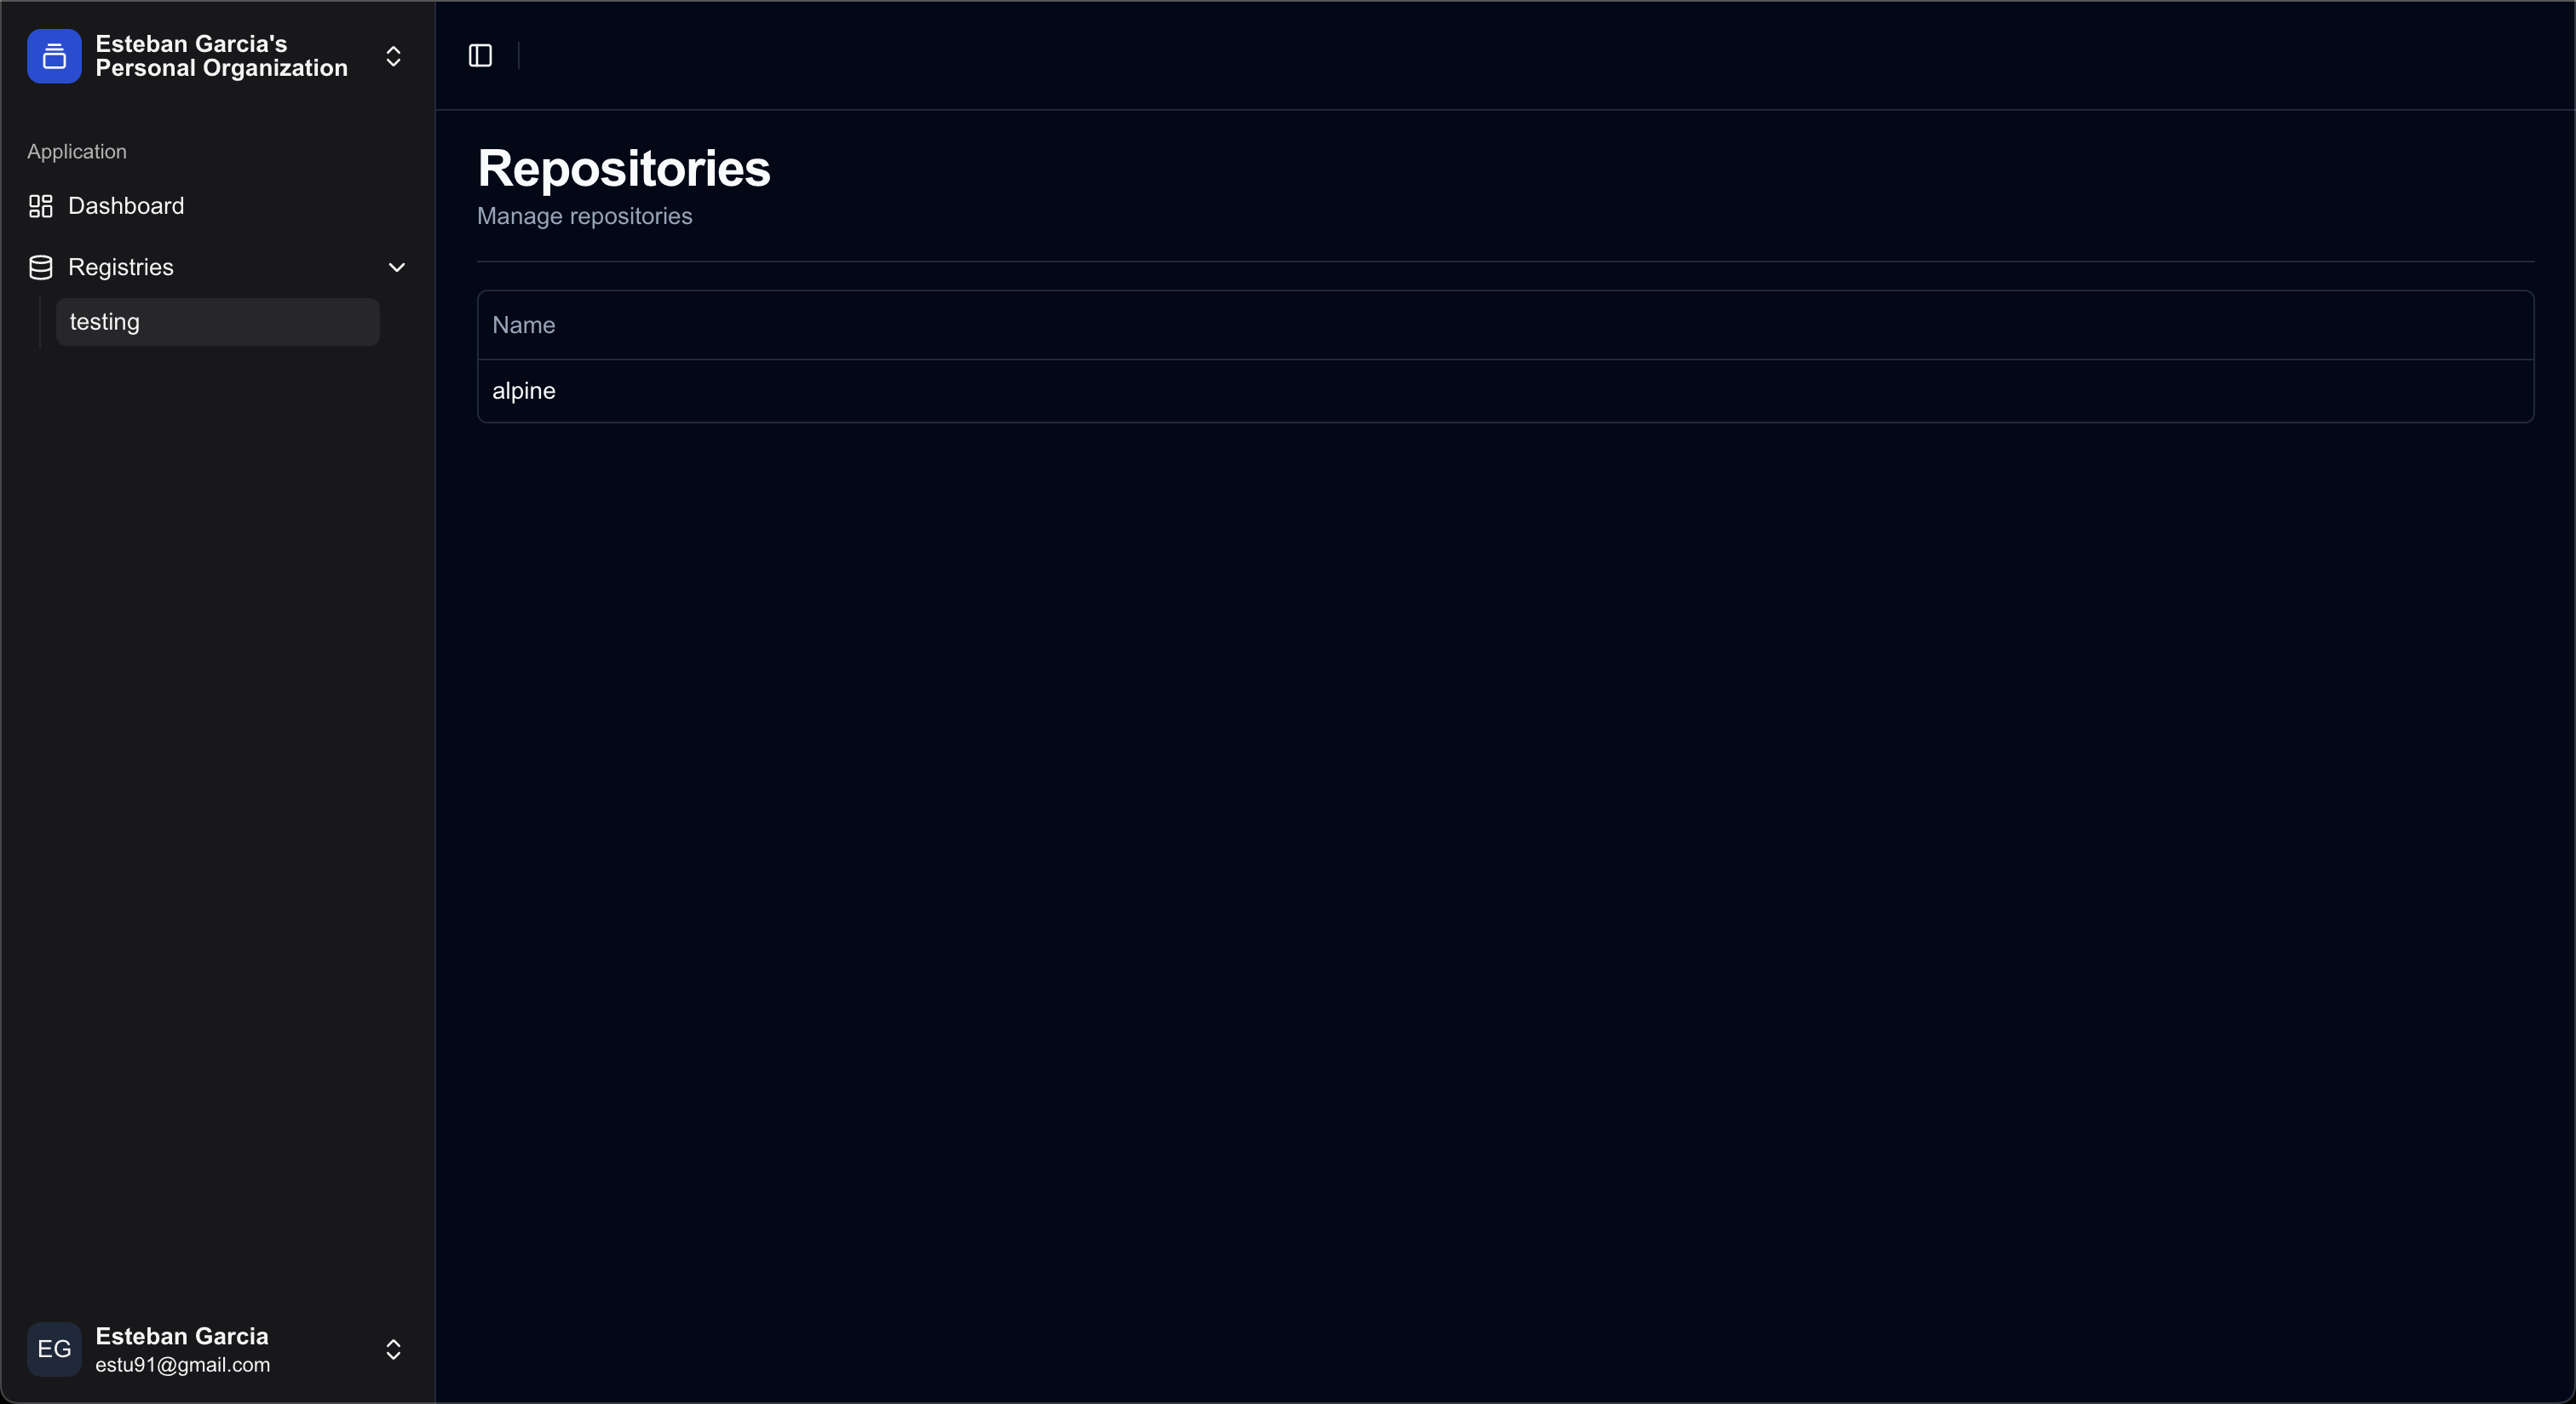
\includegraphics[scale=0.28]{screenshots/repositories.png}

  \subsection{Appendix N. OCI Conformance Tests}
  \label{sec:appendix-n}

  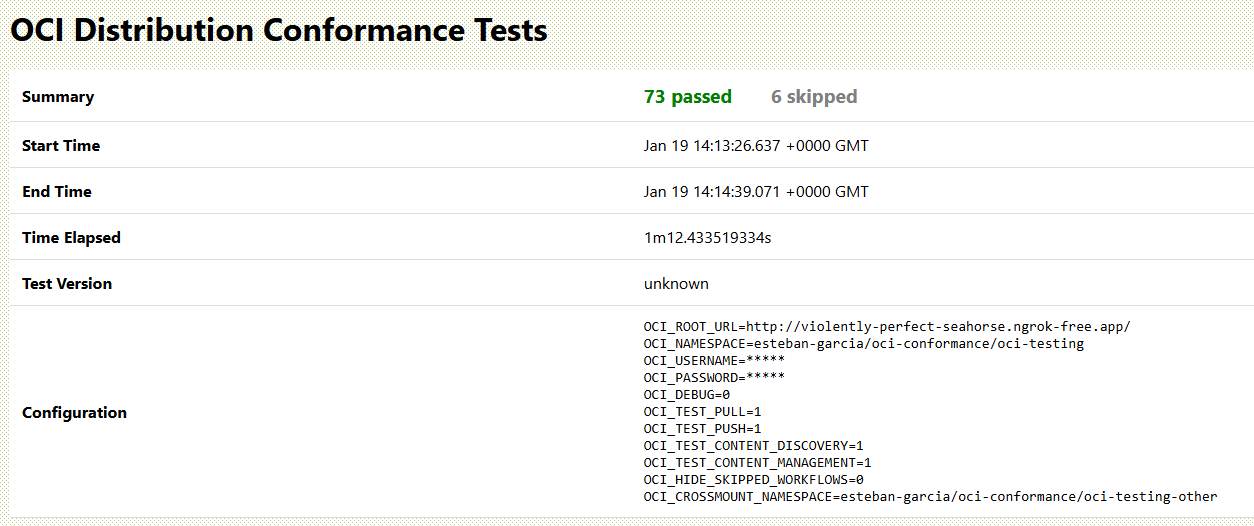
\includegraphics[scale=0.45]{appendix/oci-comformance-test.png}

\end{document}
